\chapter{Le reti di funi}

\section{Le reti di funi nell'ingegneria edile e civile}\label{chap:capitolo11}

\subsection{Reti di sicurezza}
Nell'ambito della sicurezza nei luoghi di lavoro, sono state sviluppate diverse tecnologie per la protezione degli operatori dal rischio di caduta dall'alto. Tra i Dispositivi di Protezione Collettiva (DPC), un ruolo di primario rilievo è occupato dalle reti di sicurezza (\textit{safety nets}). 

Nelle costruzioni edili e nelle opere d'ingegneria civile, le reti di sicurezza vengono impiegate sia come sistemi di arresto caduta, sia come protezioni laterali nelle lavorazioni in quota, nelle opere di riparazione delle coperture e nelle attività su ponteggi. In generale, tali reti rappresentano una soluzione altamente flessibile ed economica per mitigare i rischi legati alle cadute dall'alto. 

Rispetto ai Dispositivi di Protezione Individuale (DPI), le reti di sicurezza offrono il vantaggio di non limitare la libertà di movimento degli operatori all'interno dell'area di lavoro. Inoltre, garantiscono una cattura del corpo impattante decisamente più progressiva grazie all'elevata capacità dissipativa e deformabile del sistema. In questo modo è possibile ridurre significativamente la forza di arresto trasmessa all'operatore, mitigando anche i rischi di lesioni da trauma da impatto. 

La progettazione, il dimensionamento e la posa in opera delle reti di sicurezza in ambito europeo sono disciplinati dalla normativa \textit{EN 1263}, articolata in due parti principali: 
\begin{itemize}
    \item \text{EN 1263-1} \cite{EN1263-1}: definisce le caratteristiche dei materiali, i requisiti prestazionali dei filati e dei dispositivi che insieme alla rete costituiscono il sistema di sicurezza, oltre alle metodologie di prova di assorbimento dell'energia di deformazione e della prova dinamica. Aspetto fondamentale trattato riguarda la caratterizzazione degli effetti sulle caratteristiche meccaniche prodotte dall'invecchiamento e dall'esposizione ad azioni che provocano deterioramento. 
    \item \text{EN 1263-2} \cite{EN1263-2}: stabilisce i criteri di sicurezza per la posa in opera, definendo i limiti geometrici di caduta, i sistemi di ancoraggio ammessi e le distanze minime di spazio libero sottostante. 
\end{itemize}

In conformità con la norma \cite{EN1263-1} si identificano quattro diversi sistemi di reti di sicurezza: 
\begin{itemize}
    \item \textit{Sistema S:} Rete provvista di corda perimetrale per uso orizzontale (\cref{fig:sistema_s_norma}).  
    \item \textit{Sistema T:} Rete montata su consolle a sbalzo per uso verticale (\cref{fig:sistema_t_norma}). 
    \item \textit{Sistema U:} Rete applicata verticalmente a una struttura di supporto (\cref{fig:sistema_u_norma}).
    \item \textit{Sistema V:} Rete installata su supporto costituito da montanti a sbalzo (\cref{fig:sistema_v_norma}).
\end{itemize}

\begin{figure}[H]
    \centering
    \begin{subfigure}[b]{0.45\textwidth}
        \centering
        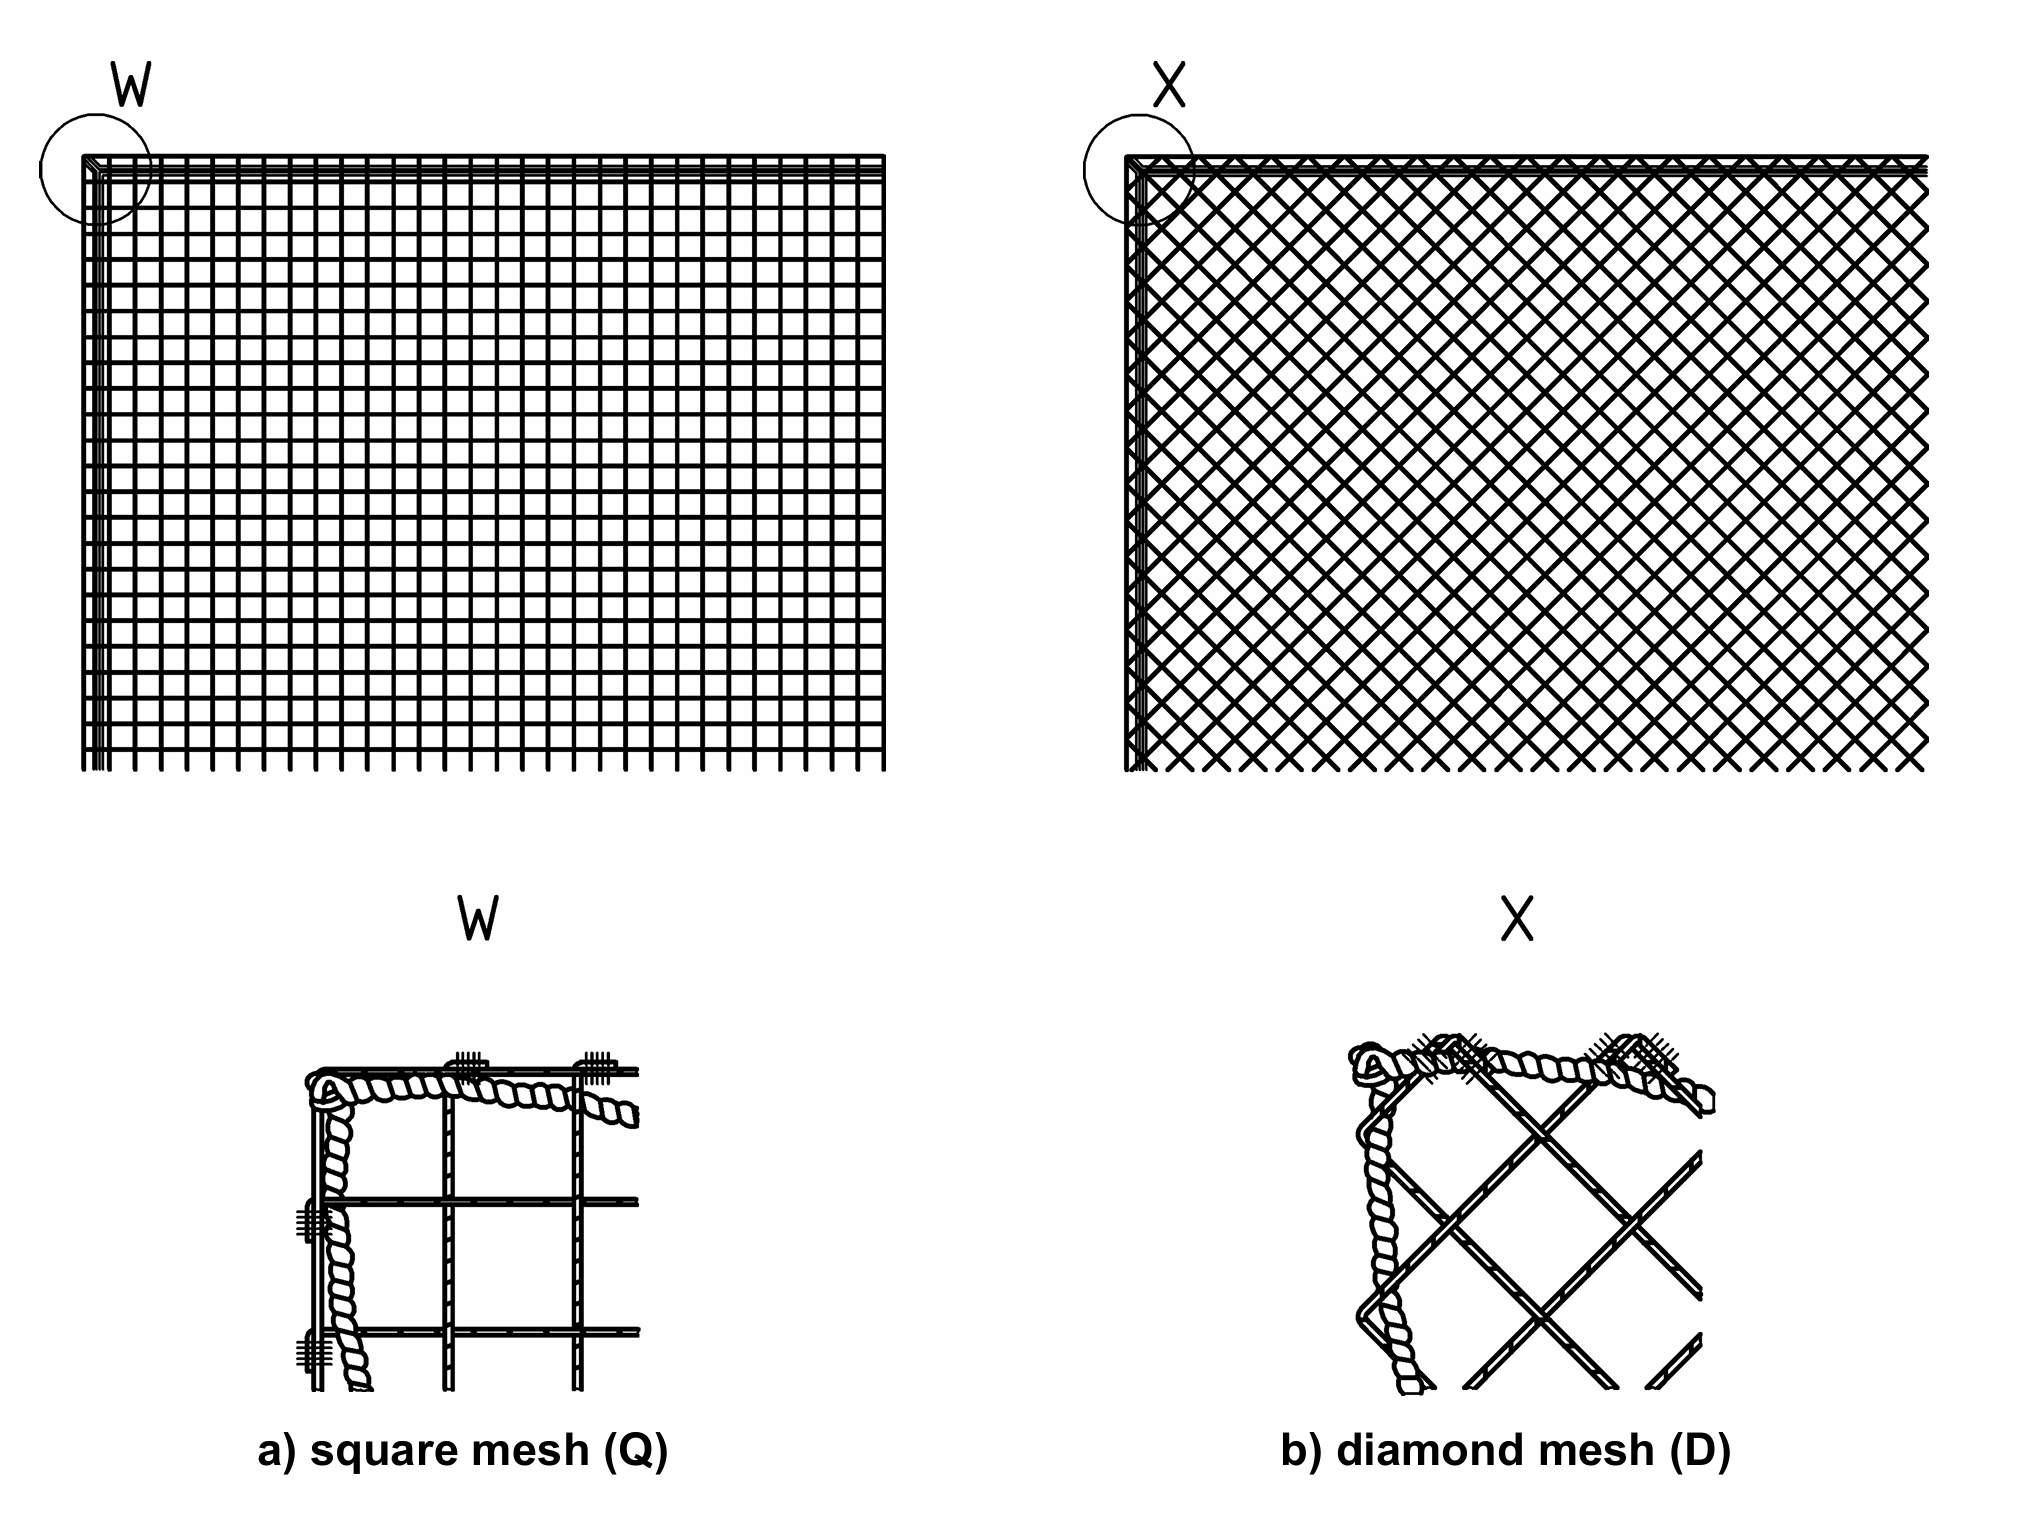
\includegraphics[height=6cm, width=\textwidth, keepaspectratio]{143_capitoli/capitolo1/immagini_capitolo_1/sistema_s.png}
        \caption{Sistema S}
        \label{fig:sistema_s_norma}
    \end{subfigure}
    \hfill
    \begin{subfigure}[b]{0.45\textwidth}
        \centering
        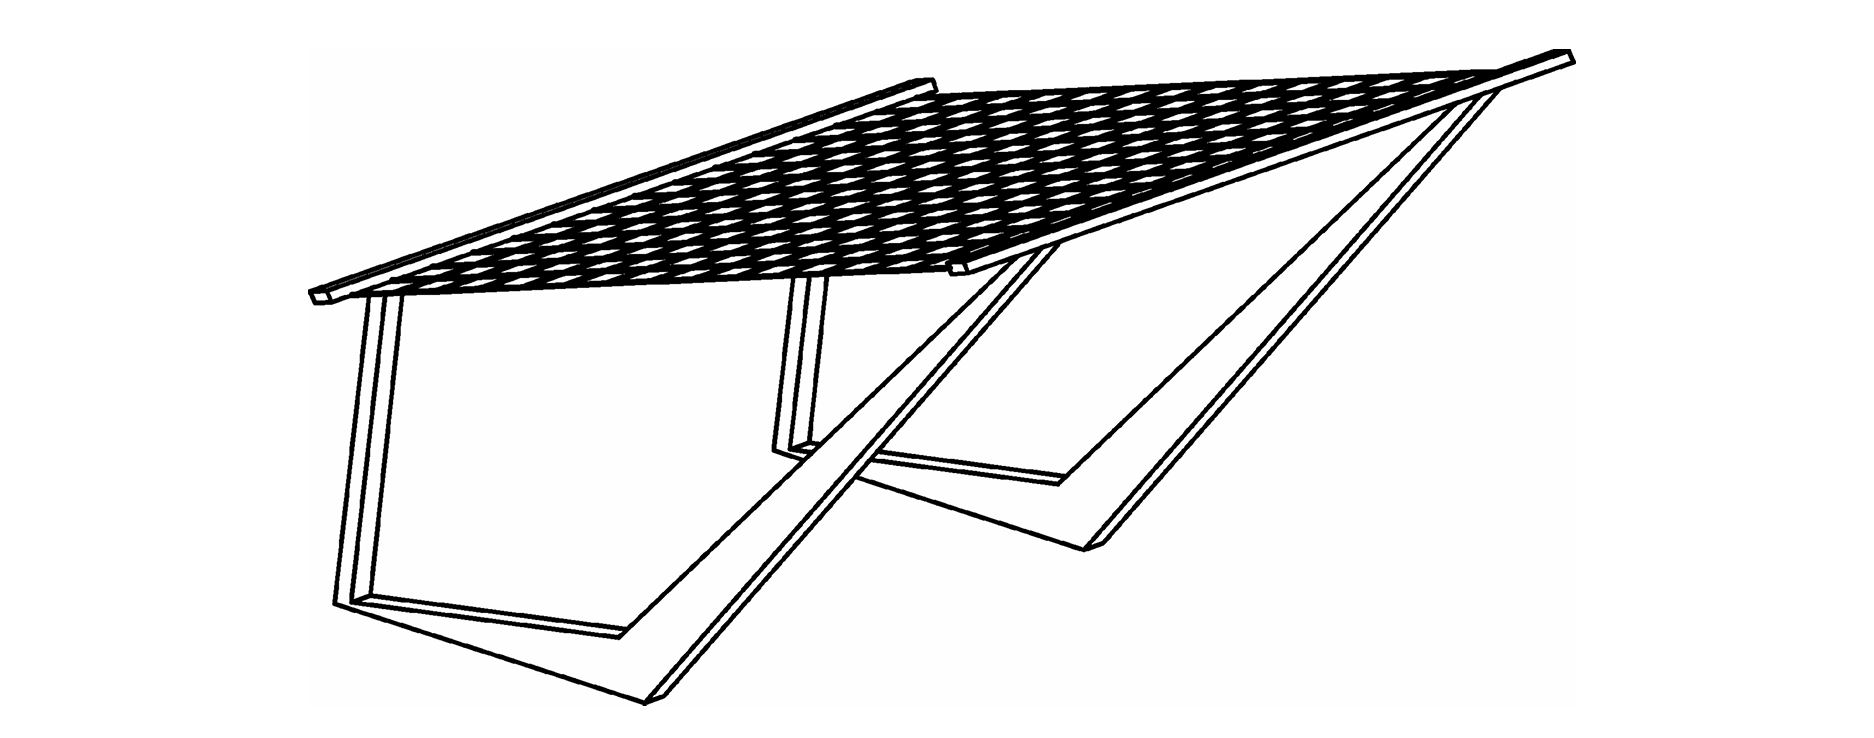
\includegraphics[height=6cm, width=\textwidth, keepaspectratio]{143_capitoli/capitolo1/immagini_capitolo_1/sistema_t.png}
        \caption{Sistema T}
        \label{fig:sistema_t_norma}
    \end{subfigure}

    \vspace{0.5cm}
    
    \begin{subfigure}[b]{0.45\textwidth}
        \centering
        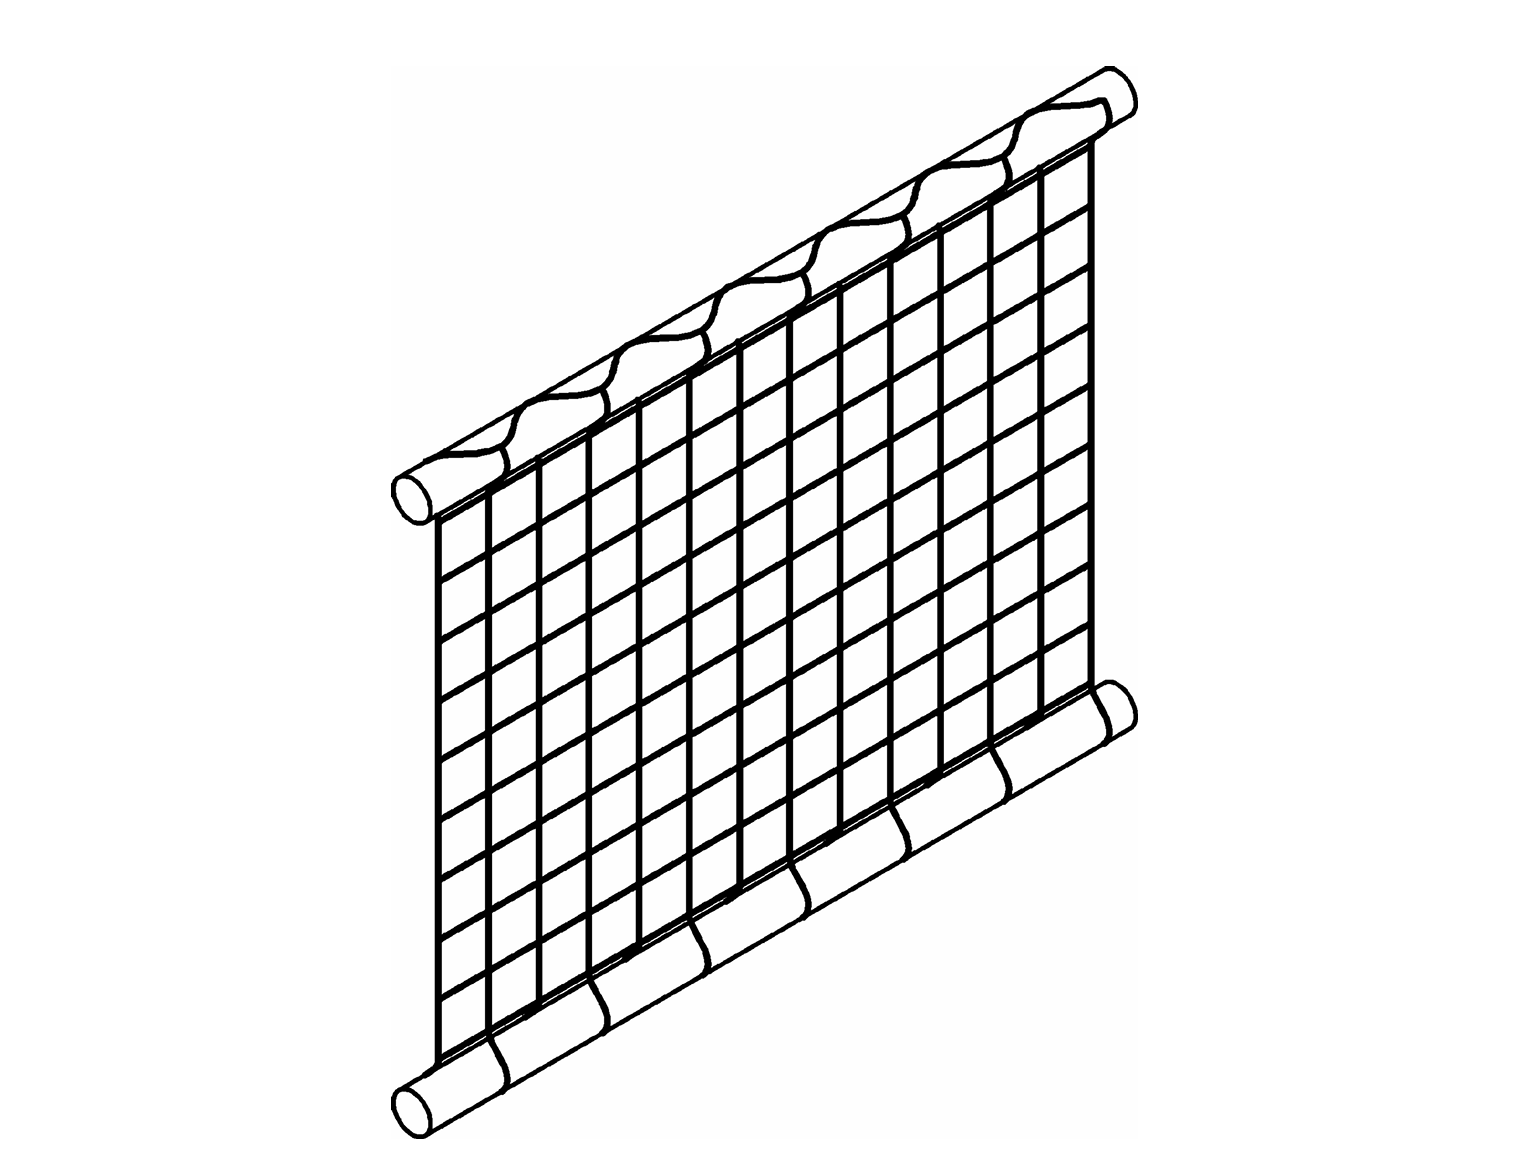
\includegraphics[height=6cm, width=\textwidth, keepaspectratio]{143_capitoli/capitolo1/immagini_capitolo_1/sistema_U.png}
        \caption{Sistema U}
        \label{fig:sistema_u_norma}
    \end{subfigure}
    \hfill
    \begin{subfigure}[b]{0.45\textwidth}
        \centering
        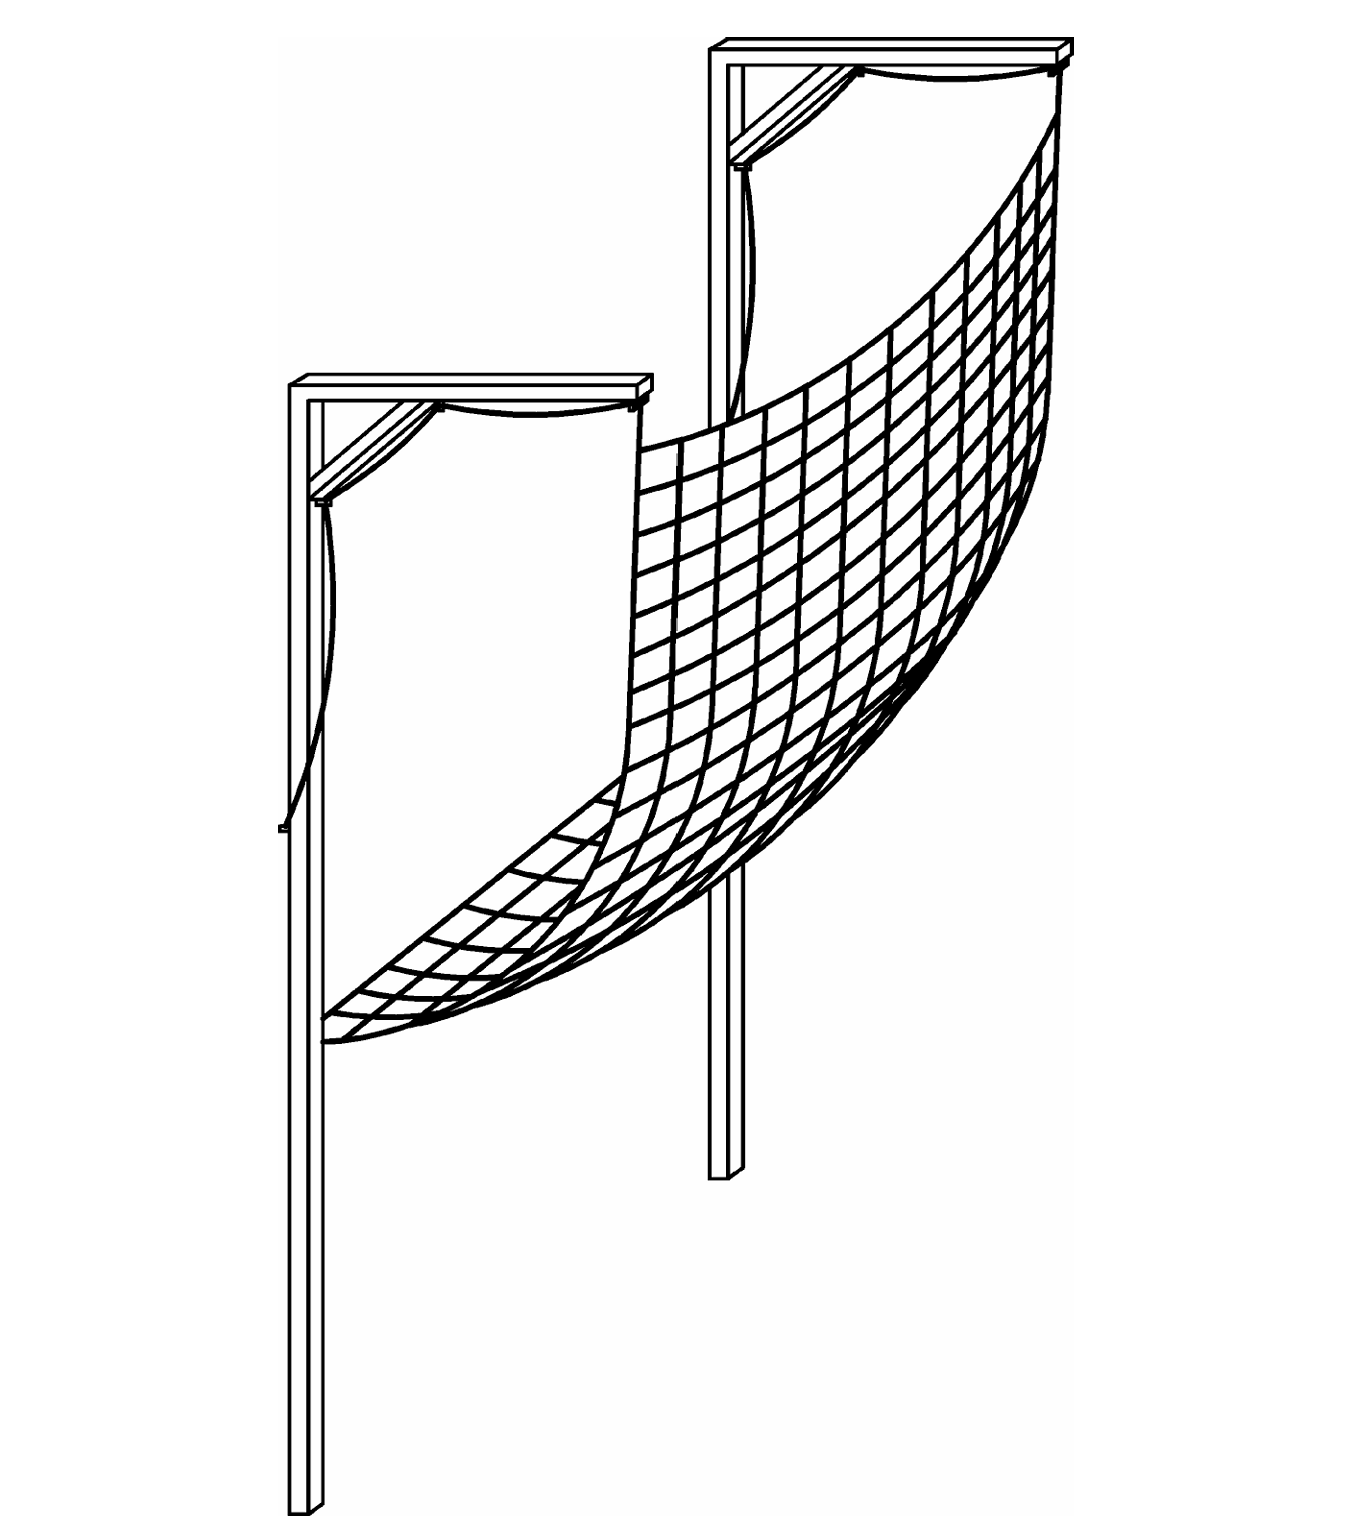
\includegraphics[height=6cm, width=\textwidth, keepaspectratio]{143_capitoli/capitolo1/immagini_capitolo_1/sistema_v.png}
        \caption{Sistema V}
        \label{fig:sistema_v_norma}
    \end{subfigure}

    \caption{Classificazione dei quattro sistemi di reti di sicurezza secondo la norma EN 1263-1. Fonte: BS EN 1263-1}
    \label{fig:sistemi_reti_norma}
\end{figure}

\subsubsection{Sistema S}
Il sistema di sicurezza tipo S è tra quelli regolati in \cite{EN1263-1} il cui comportamento è maggiormente svincolato da strutture esterne. Difatti, consta di una rete bordata da una fune perimetrale (\textit{border rope}) alla quale si collegano le funi di ancoraggio (\textit{tie rope}) per il vincolo alle strutture portanti. Tale sistema è installato prevalentemente in posizione orizzontale per coprire ampie superfici sottostanti la zona di lavoro (ad esempio nella prevenzione delle cadute durante la costruzione di solai, tetti o vani interni).

Il meccanismo di dissipazione energetica del Sistema S si basa sul comportamento della rete: l'energia cinetica del corpo impattante viene convertita prevalentemente in lavoro di deformazione elastoplastica e viscoelastica delle maglie e in sforzi di trazione lungo le funi di bordo e di ancoraggio. Per questo motivo, l'applicazione del sistema richiede una rigorosa valutazione dello spazio libero sottostante, onde evitare che la freccia d'inflessione massima raggiunga ostacoli o il piano di calpestio sottostante durante l'impatto.

La norma \cite{EN1263-1} si applica esclusivamente a reti con superficie coperta non inferiore a $35 \, \text{m}^2$, e, nel caso di superficie rettangolare, con lato minore di almento $5.0 \, \text{m}$. Qualora la superficie da proteggere risulti inferiore a tali limiti dimensionali, il campo di applicazione della norma europea viene demandato ai rispettivi regolamenti nazionali; in Italia, la progettazione, la prova e la posa di tali dispositivi di piccole dimensioni sono disciplinate dalla normativa nazionale UNI 11808, articolata nella \cite{UNI11808-1} per reti rettangolari con lato cordo da $3\,\text{m}$ a $5\,\text{m}$ e nella \cite{UNI11808-2} per reti rettangolari con lato corto da $2\,\text{m}$ a $3\,\text{m}$.

Nel caso in cui sia necessario coprire estensioni superficiali superiori mediante l'unione di più reti adiacenti, la norma \cite{EN1263-2} prescrive due modalità alternative di accoppiamento: la guinzione tramite fune di accoppiamento (\textit{coupling rope}), assicurando che non si creino aperture con luce superiore a $100 \, \text{mm}$ tra i bordi, oppure il collegamento per semplice sovrapposizione, per il quale è richiesta una larghezza di sovrapposizione minima pari ad almeno $2.0 \, \text{m}$.

\begin{figure}[htbp]
    \centering
    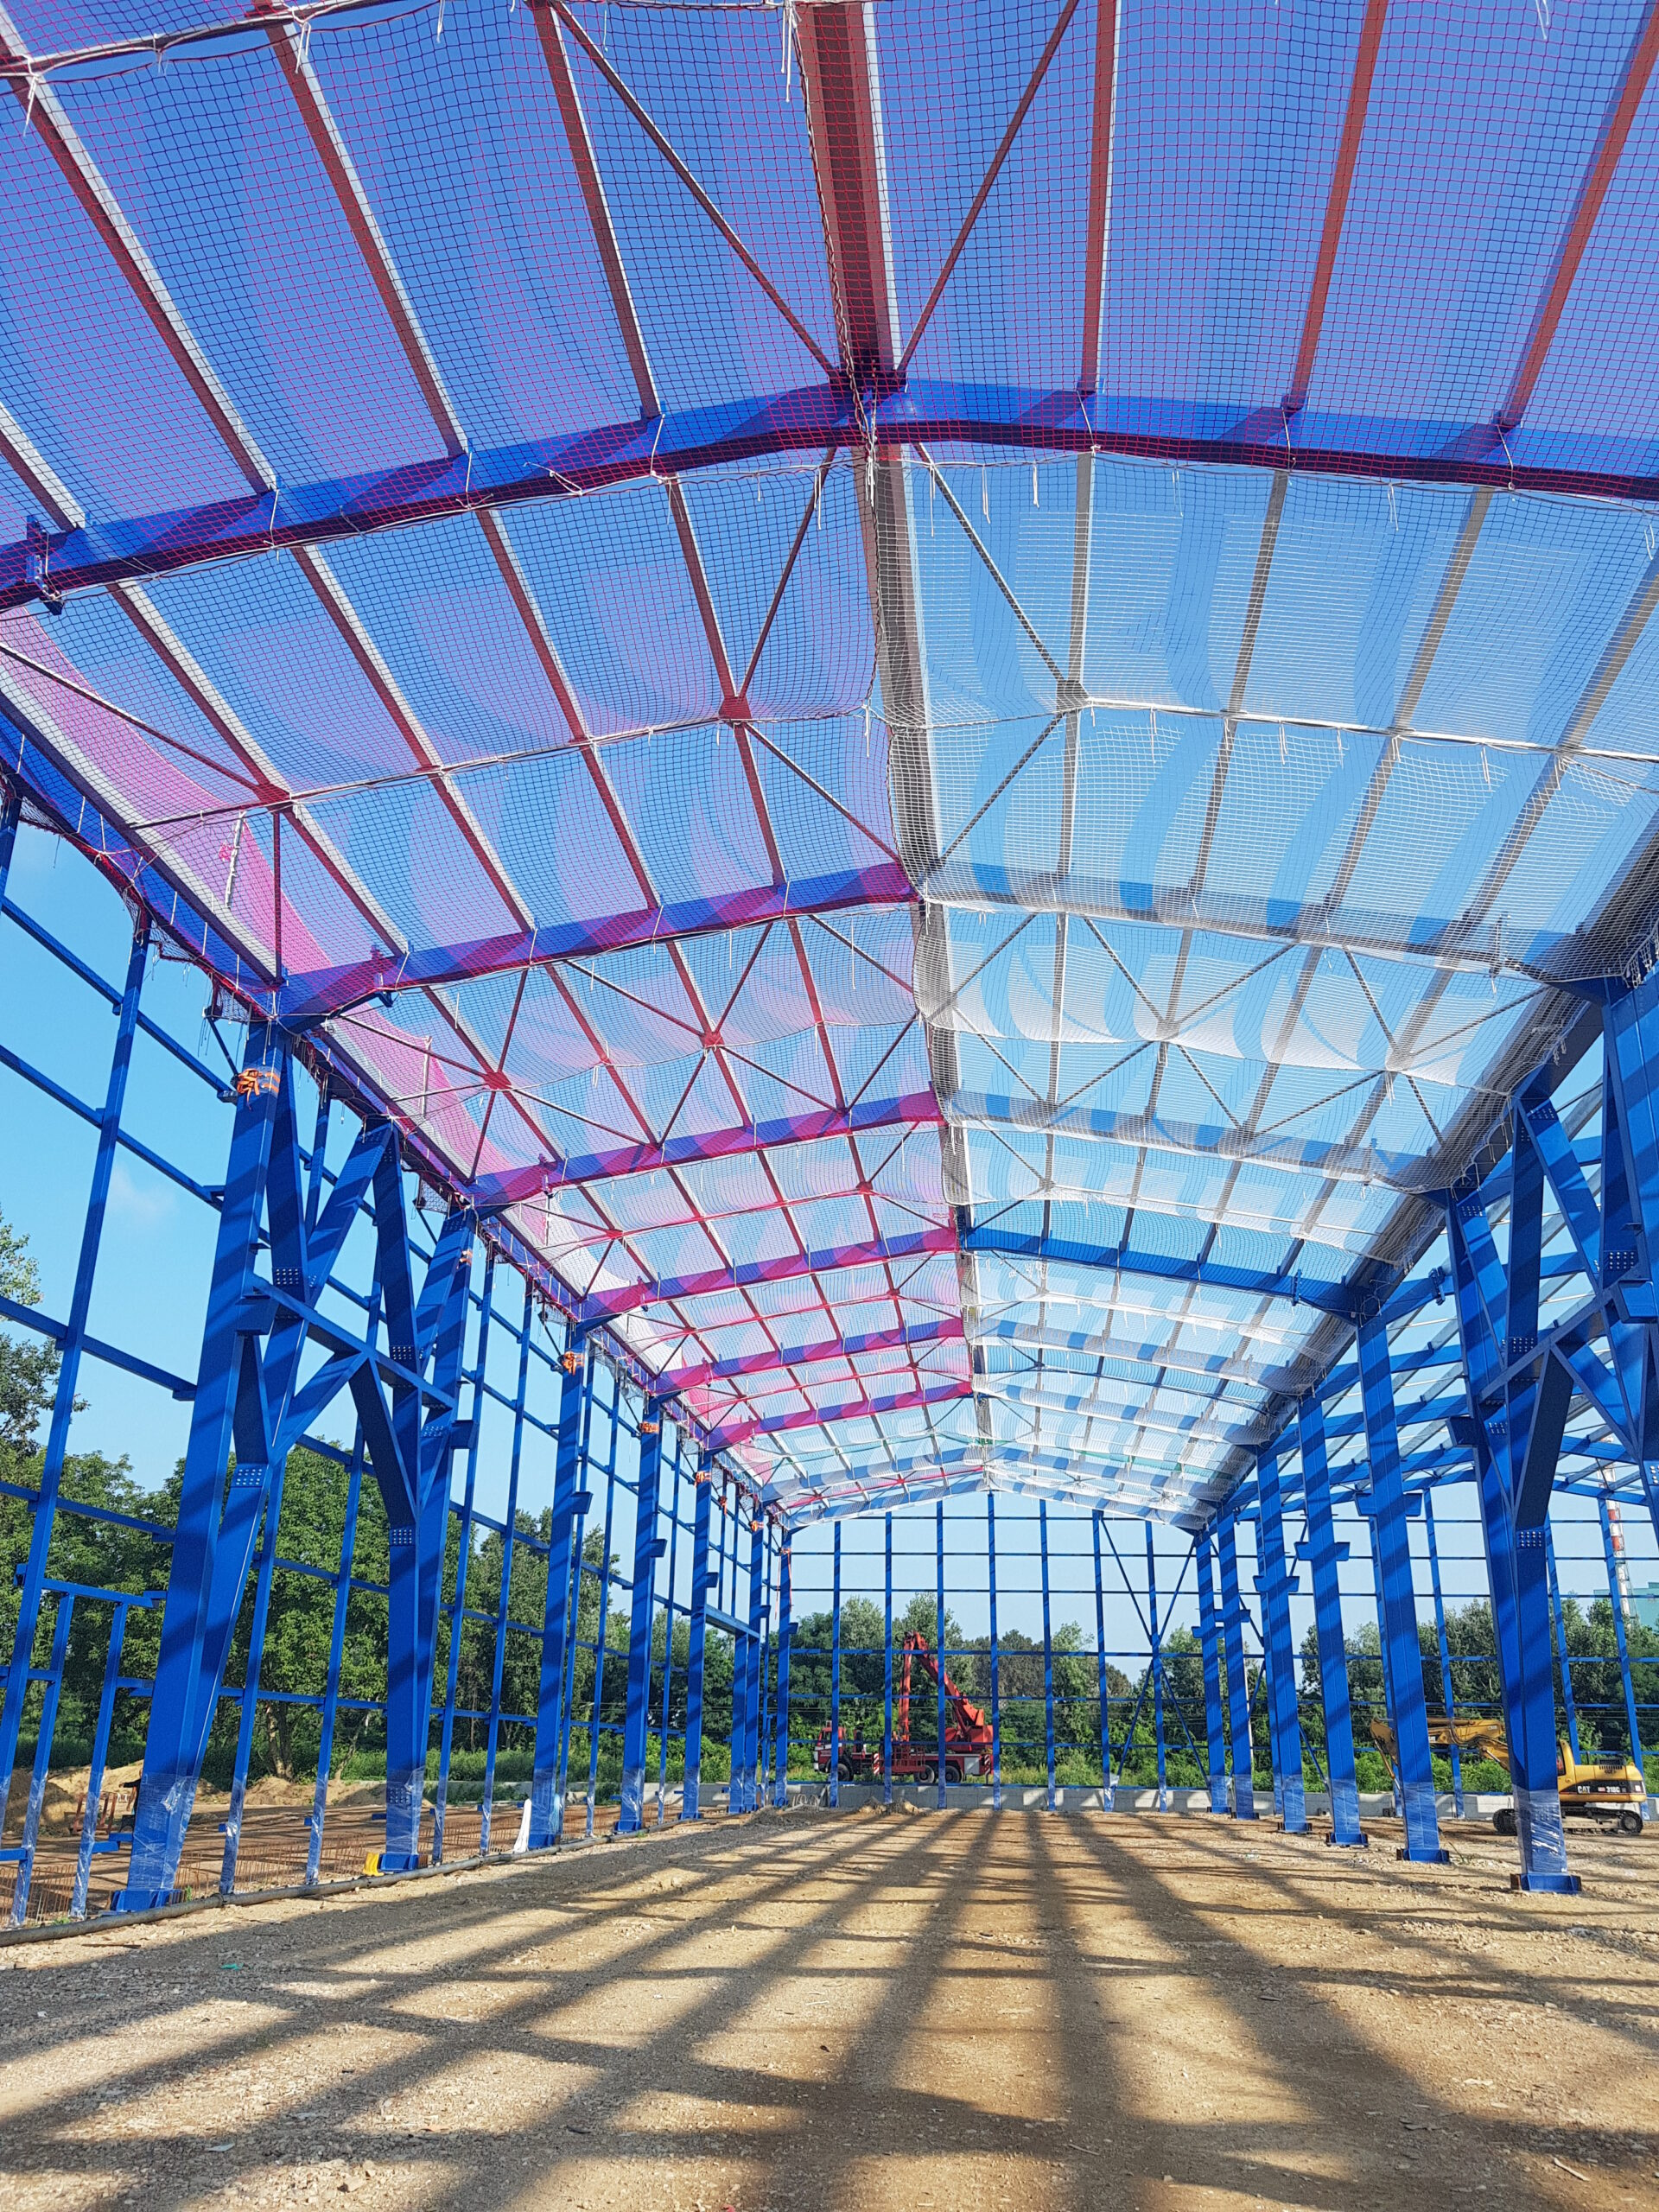
\includegraphics[height=0.35\textheight, keepaspectratio]{143_capitoli/capitolo1/immagini_capitolo_1/sistema_s_figura.png}
    \caption{Applicazione di un Sistema S su struttura in acciaio. Fonte: www.laretesrl.it}
    \label{fig:sistema_s_figura}
\end{figure}

\subsubsection{Sistema T}
Il sistema di sicurezza tipo T prevede che la rete sia montata su apposite consolle metalliche a sbalzo ancorate alla struttura portante dell'edificio. Tale configurazione crea un piano di protezione orizzontale aggettante verso l'esterno del bordo del fabbricato, con lo scopo di intercettare persone o materiali in caduta dai livelli di lavoro superiori.

Dal punto di vista del comportamento meccanico, il Sistema T costituisce una struttura di arresto mista: la dissipazione dell'energia cinetica del corpo impattante si ripartisce tra la deformazione elastoplastica e viscoelastica delle maglie della rete e la risposta flessionale della consolle di supporto.

In conformità con \cite{EN1263-2}, la geometria del piano di protezione - ossia la larghezza dell'aggetto $b$ - è strettamente vincolata all'altezza di caduta libera ammissibile ($h$). Per altezze di caduta fino a $3.0 \, \text{m}$, l'aggetto minimo della consolle deve essere pari a $3.0 \, \text{m}$; la norma consente altezze di caduta massime fino a $h = 6.0 \, \text{m}$, a condizione che la larghezza di cattura del piano aggettante rimanga commisurata alla freccia massima della parabola di caduta.

Dal punto di vista operativo, i moduli del Sistema T presentano vantaggi in termini di modularità e riposizionabilità: le consolle possono essere sollevate e riancorate ai piani superiori durante l'avanzamento dei solai (sistemi rampanti). La continuità della protezione lungo lo sviluppo della facciata deve essere garantita unendo le reti dei singoli moduli adiacenti tramite funi di accoppiamento (\textit{coupling rope}) assicurando che non si formino aperture con luce superiore a $100 \, \text{mm}$ tra i bordi, oppure, nel caso in cui il collegamento avvenga per sovrapposizione, garantendo una larghezza di sovrapposizione minima pari ad almeno $0.75 \, \text{m}$.

\begin{figure}[htbp]
    \centering
    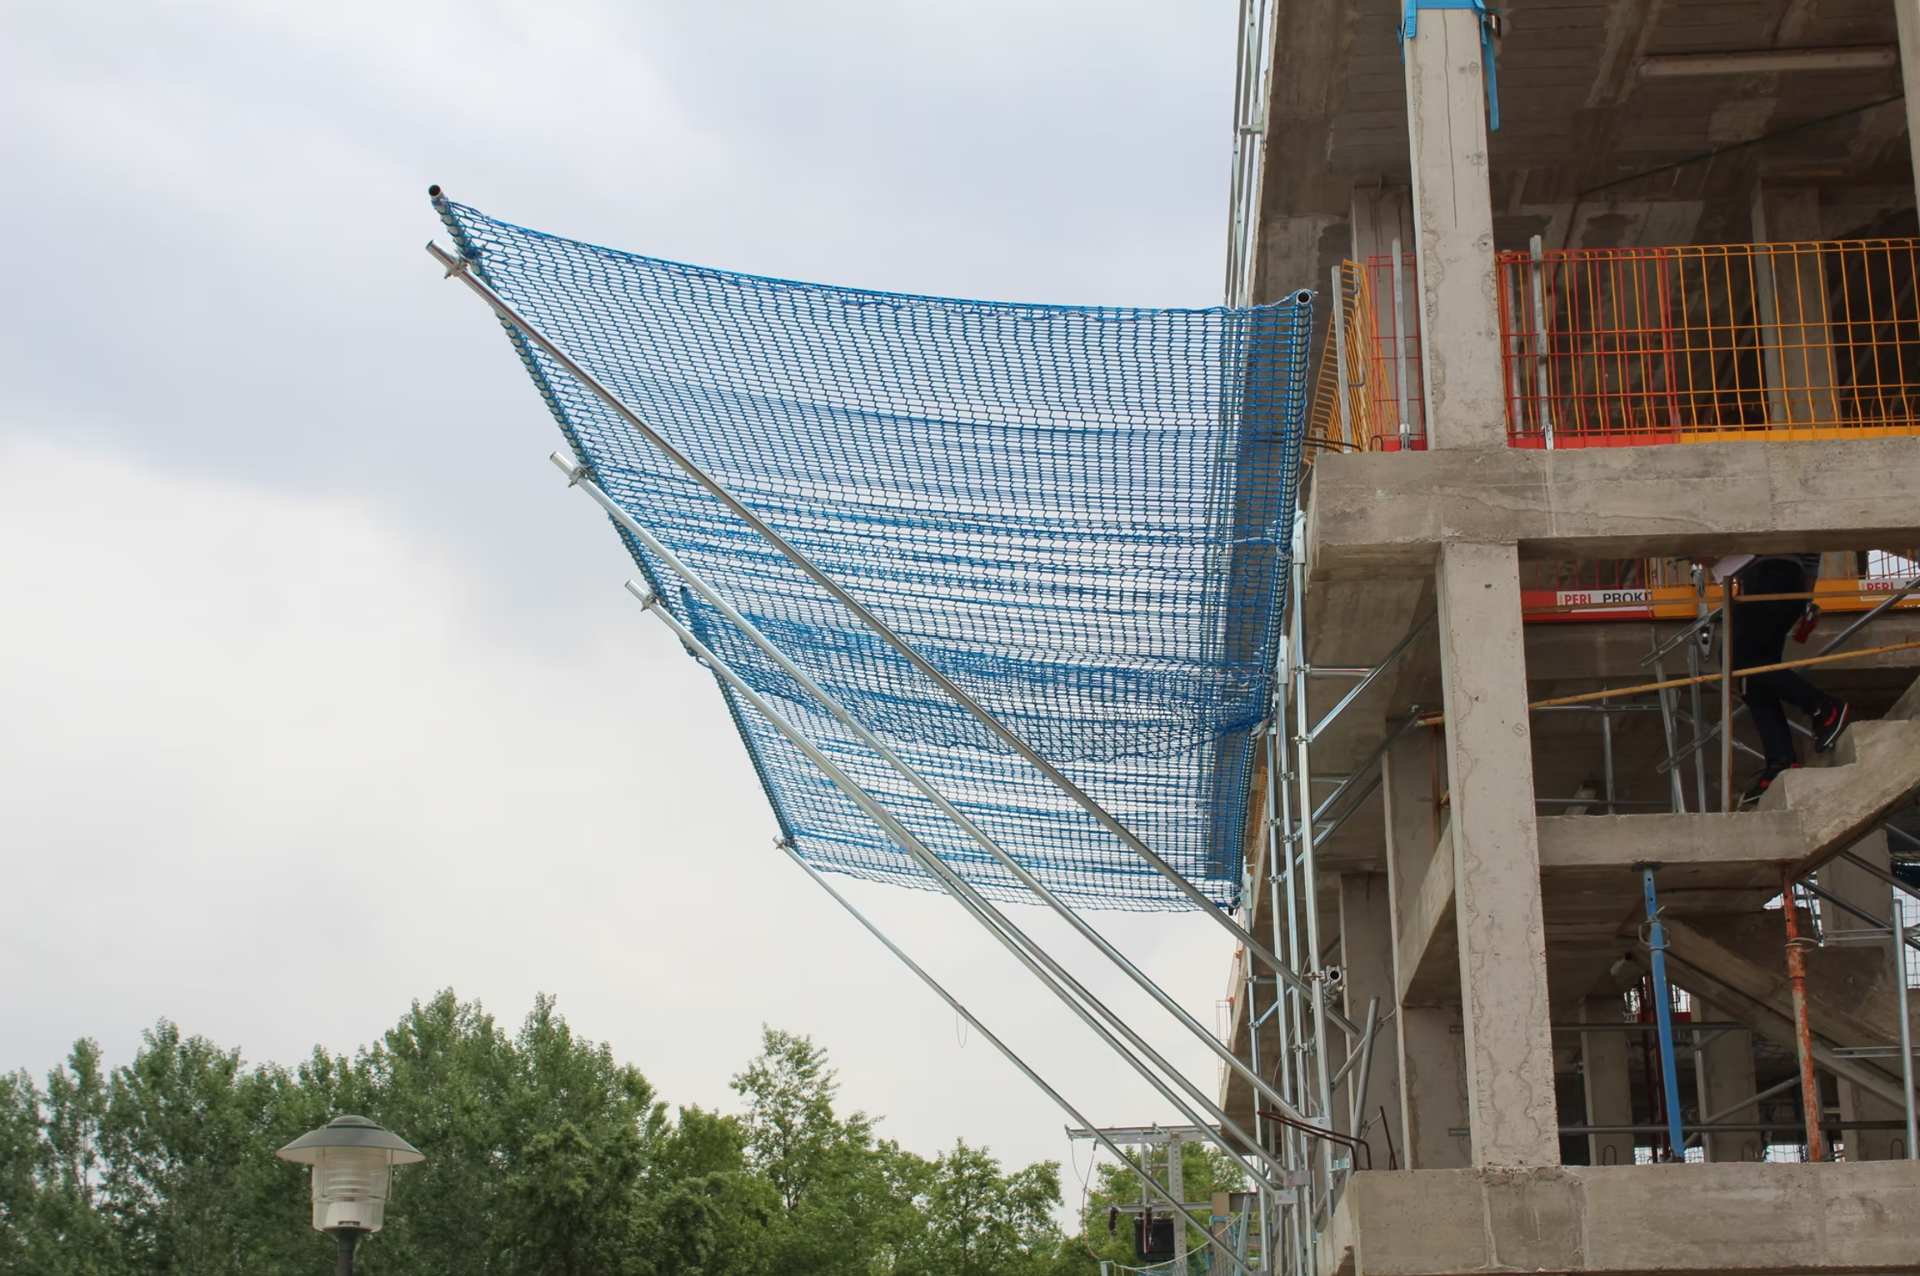
\includegraphics[height=0.35\textheight, keepaspectratio]{143_capitoli/capitolo1/immagini_capitolo_1/sistema_t_figura.png}
    \caption{Applicazione di un Sistema T su struttura a talaio in calcestruzzo armato. Fonte: www.retibrembo.com}
    \label{fig:sistema_t_figura}
\end{figure}

\subsubsection{Sistema U}
Nei sistemi U la rete di sicurezza viene applicata in posizione verticale vincolata ad una struttura portante di supporto. Il sistema U è concepito prevalentemente come protezione di bordo o protezione temporanea laterale, installata lungo i perimetri dei piani di lavoro, sulle coperture inclinate o integrata nei ponteggi di cantiere. Quando impiegato per la chiusura dei bordi perimetrici sottoposti ad impatti dinamici, l'inquadramento prestazionale di tali dispositivi è regolato sia dalle norme sulle reti di protezione \cite{EN1263-2} sia dalla normativa sui sistemi temporanei di protezione di bordo \cite{EN13374-2025} (in particolare per i sistemi di Classe C, progettati per assorbire energia di impatto fino a $2.2 \, \text{kJ}$).

Sebbene il sistema U nasca per un'applicazione prevalentemente verticale, il comportamento dinamico e le prestazioni dissipative della sola rete di sicurezza in tali configurazioni sono stati approfonditamente analizzati nell'ambito dello studio dei \textit{temporary edge protection system} da Pomares Torres et al.\cite{Pomares2011} attraverso modellazioni numeriche agli elementi finiti. 
\begin{figure}[htbp]
    \centering
    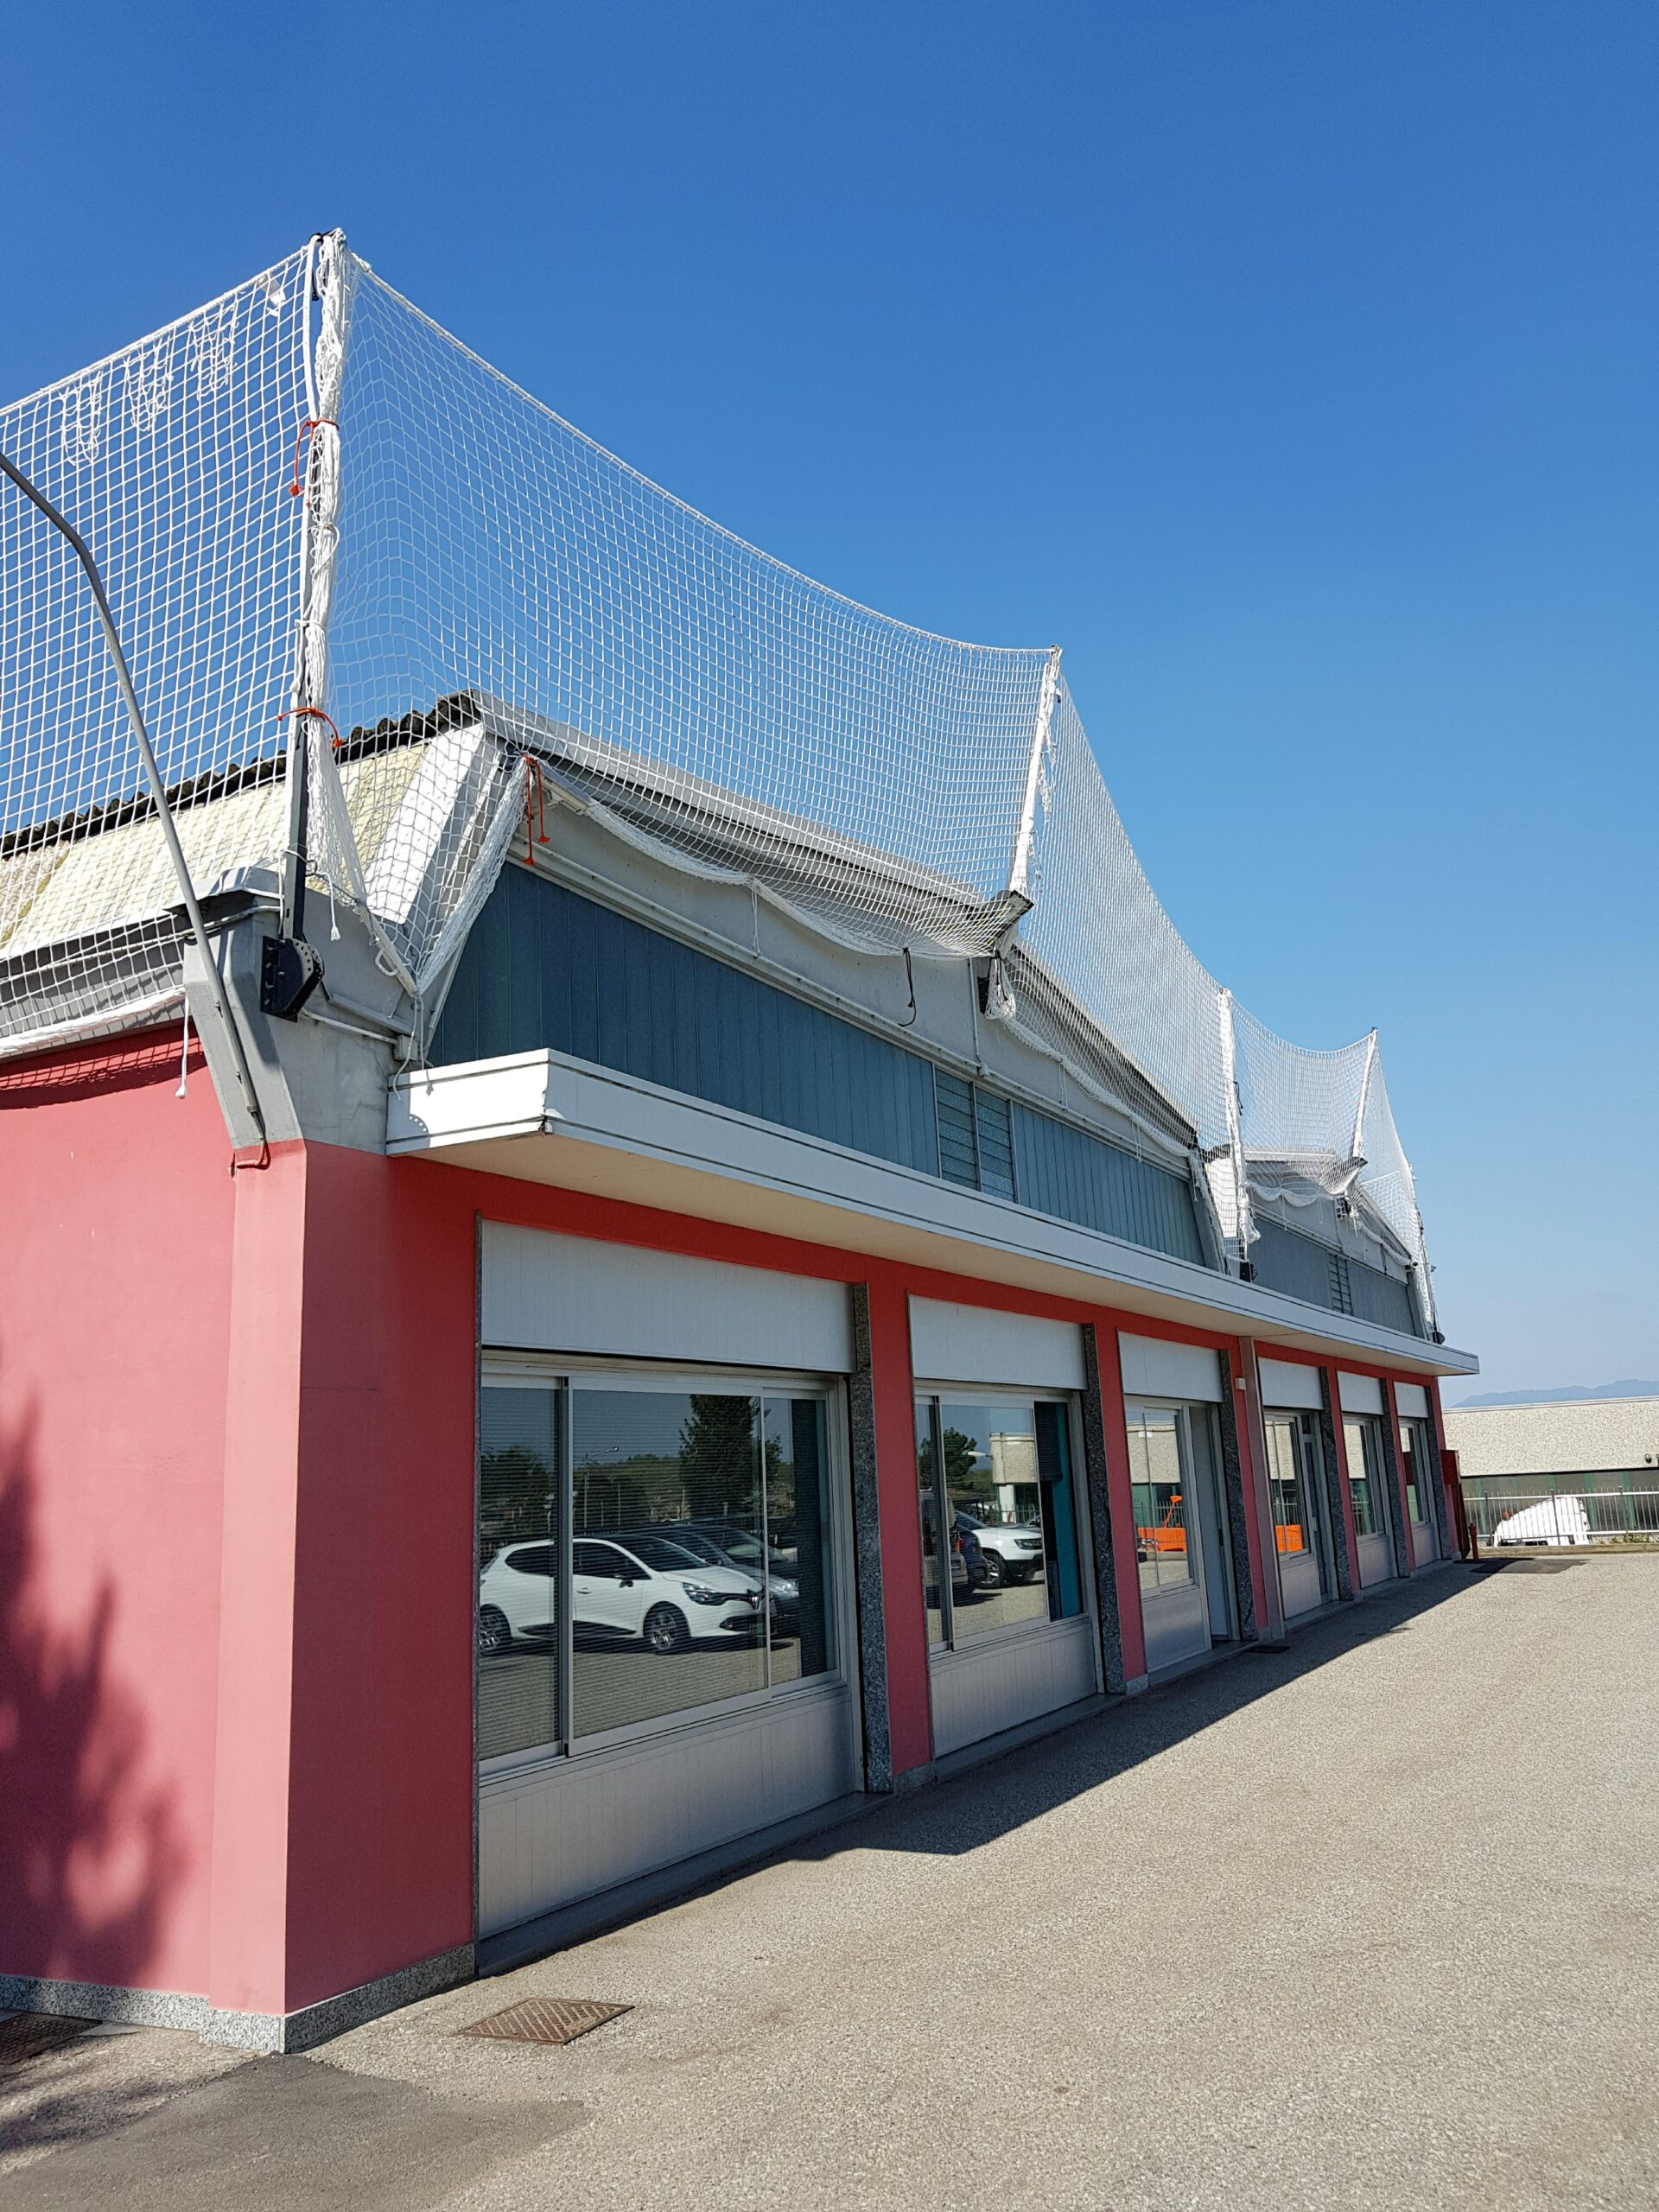
\includegraphics[height=0.35\textheight, keepaspectratio]{143_capitoli/capitolo1/immagini_capitolo_1/sistema_u_figura.png}
    \caption{Applicazione di un Sistema U. Fonte: www.laretesrl.it}
    \label{fig:sistema_u_figura}
\end{figure}

\subsubsection{Sistema V}
Il sistema V definisce una rete di sicurezza orientata prevalentemenete in direzione verticale, vincolata a un supporto con montante a sbalzo, in conformità con quanto previsto dalla norma \cite{EN1263-1}.

A differenza dei sistemi a sviluppo orizzontale, il Sistema V presenta una forte caratterizzazione geografica per quanto riguarda l'impiego operativo, infatti, in ambito europeo la Spagna, rappresenta il contesto di massima diffusione del Sistema V. Tale primato è legato strettamente all'evoluzione della normativa nazionale sulla prevenzione dei rischi lavorativi ed alle prassi costruttive tipiche dell'edilizia residenziale spagnola. 

In virtù di questo consolidato utilizzo pratico, la maggioranza della letteratura scientifica internazionale focalizzata sulla risposta meccanica di tali sistemi proviene dagli atenei spagnoli.

Per comprendere il funzionamento del Sistema V, occorre analizzare la risposta strutturale dell'insieme rete-supporti sotto l'azione di carichi d'impatto dinamici. Il comportamento ed i suoi difetti storici dei primi casi d'impiego sono stati identificati in \cite{Segovia2008}. Nello specifico in \cite{Segovia2008} si evidenzia come i sistemi tradizionali soffrissero di importanti criticità progettuali dovute ad una concezione errata dei supporti metallici. 

L'analisi della risposta dinamica non lineare e la caratterizzazione numerica di tale interazione sono state sviluppate in \cite{Segovia2007}. Attraverso modelli ad elementi finiti (FEM) calibrati su prove sperimentali di impatto previste da \cite{EN1263-1}, lo studio stabilisce la ripartizione dell'energia assorbita durante l'impatto: la rete di sicurezza assorbe l'$85\% - 88\%$ dell'energia totale dell'impatto ($\approx 6.8 - 7.0 \, \text{kJ}$) - principalmente per mezzo della deformazione elastoplastica dei filamenti e del serraggio dei nodi della maglia - mentre i supporti metallici assorbono il restante $11\% - 15\%$ dell'energia cinetica del corpo immediatamente precedente all'impatto ($\approx 0.77 - 0.83\, \text{kJ}$). 
\begin{figure}[htbp]
    \centering
    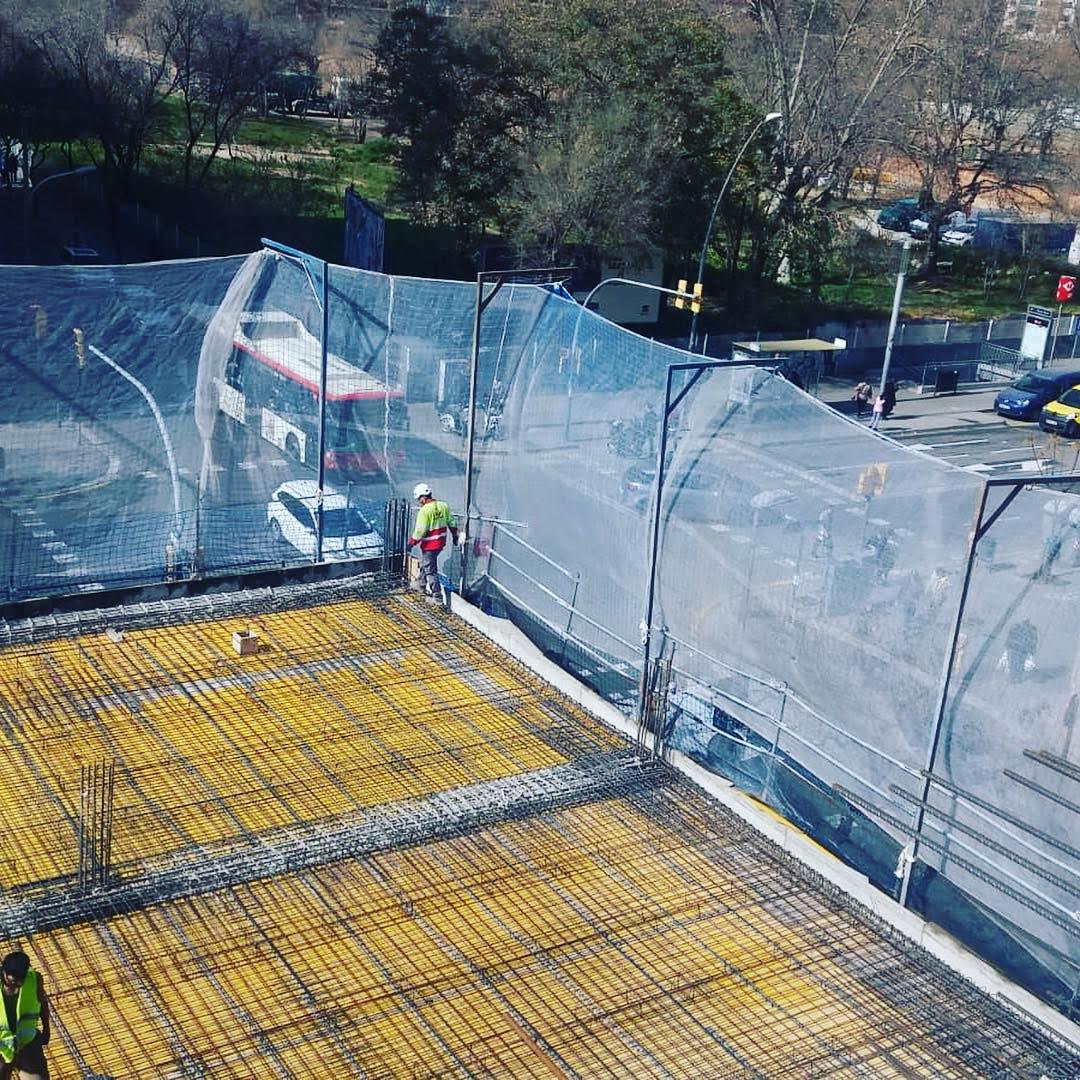
\includegraphics[height=0.35\textheight, keepaspectratio]{143_capitoli/capitolo1/immagini_capitolo_1/sistema_v_figura.png}
    \caption{Applicazione di un Sistema V su struttura a telaio in calcestruzzo armato in fase di costruzione. Fonte: www.leondeoro.com}
    \label{fig:sistema_v_figura}
\end{figure}

\subsubsection{Classificazione geometrica e costruttiva delle reti}
Oltre alla distinzione per tipologia di sistema (S, T, U, V), le reti di sicurezza sono classificate dalla norma \cite{EN1263-1} in base alla geometria della maglia e alla tecnologia di tessitura impiegata per l'unione dei filati nei nodi o nei punti di giunzione. Indipendentemente dalle prestazioni energetiche del materiale, la configurazione geometrica influisce direttamente sulla distribuzione degli sforzi e sulla flessibilità globale della rete. 

Relativamente all'orientamento ed alle dimensioni della maglia, la norma identifica due geometrie per le maglie della rete: 
\begin{itemize}
    \item \textit{Maglia quadrata (squared mesh - (Q)):} i fili costituenti la maglia sono disposti parallelamente e ortogonalmente rispetto alle funi perimetrali di bordo. Questa configurazione offre una risposta meccanica più rigida lungo le direzioni principali, riducendo le concentrazioni di tensione negli angoli ma risulta poco idonea alla trasmissione di sollecitazioni di taglio. 
    \item \textit{Maglia romboidale (diamond mesh - (D)):} i fili della maglia sono orientati con un inclinazione di $45\, ^\circ$ rispetto al perimetro della rete. Tale disposizione garantisce una maggiore deformabilità iniziale sotto carico, consentendo di sviluppare durante l'entrata in carico elevate frecce d'inflessione prima di mettere in tensione le funi. 
\end{itemize}

La dimensione nominale della maglia $l_m$ rappresenta la distanza tra due nodi consecutivi (o due giunzioni). Nei sistemi di protezione contro le cadute dall'alto la dimensioni standard più utilizzate sono $l_m = 100 \, \text{mm}$ e $l_m = 60 \, \text{mm}$. In funzione delle dimensioni massime della maglia e del valore nominale della capacità di assorbire energia elastica, la norma classifica le reti in differenti classi prestazionali; tale classificazione verrà presentata successivamente nel \cref{chap:capitolo3}, unitamente alle modalità prevista dalla normativa per la valutazione dell'energia assorbibile dalla rete.  
\begin{figure}[htbp]
    \centering
    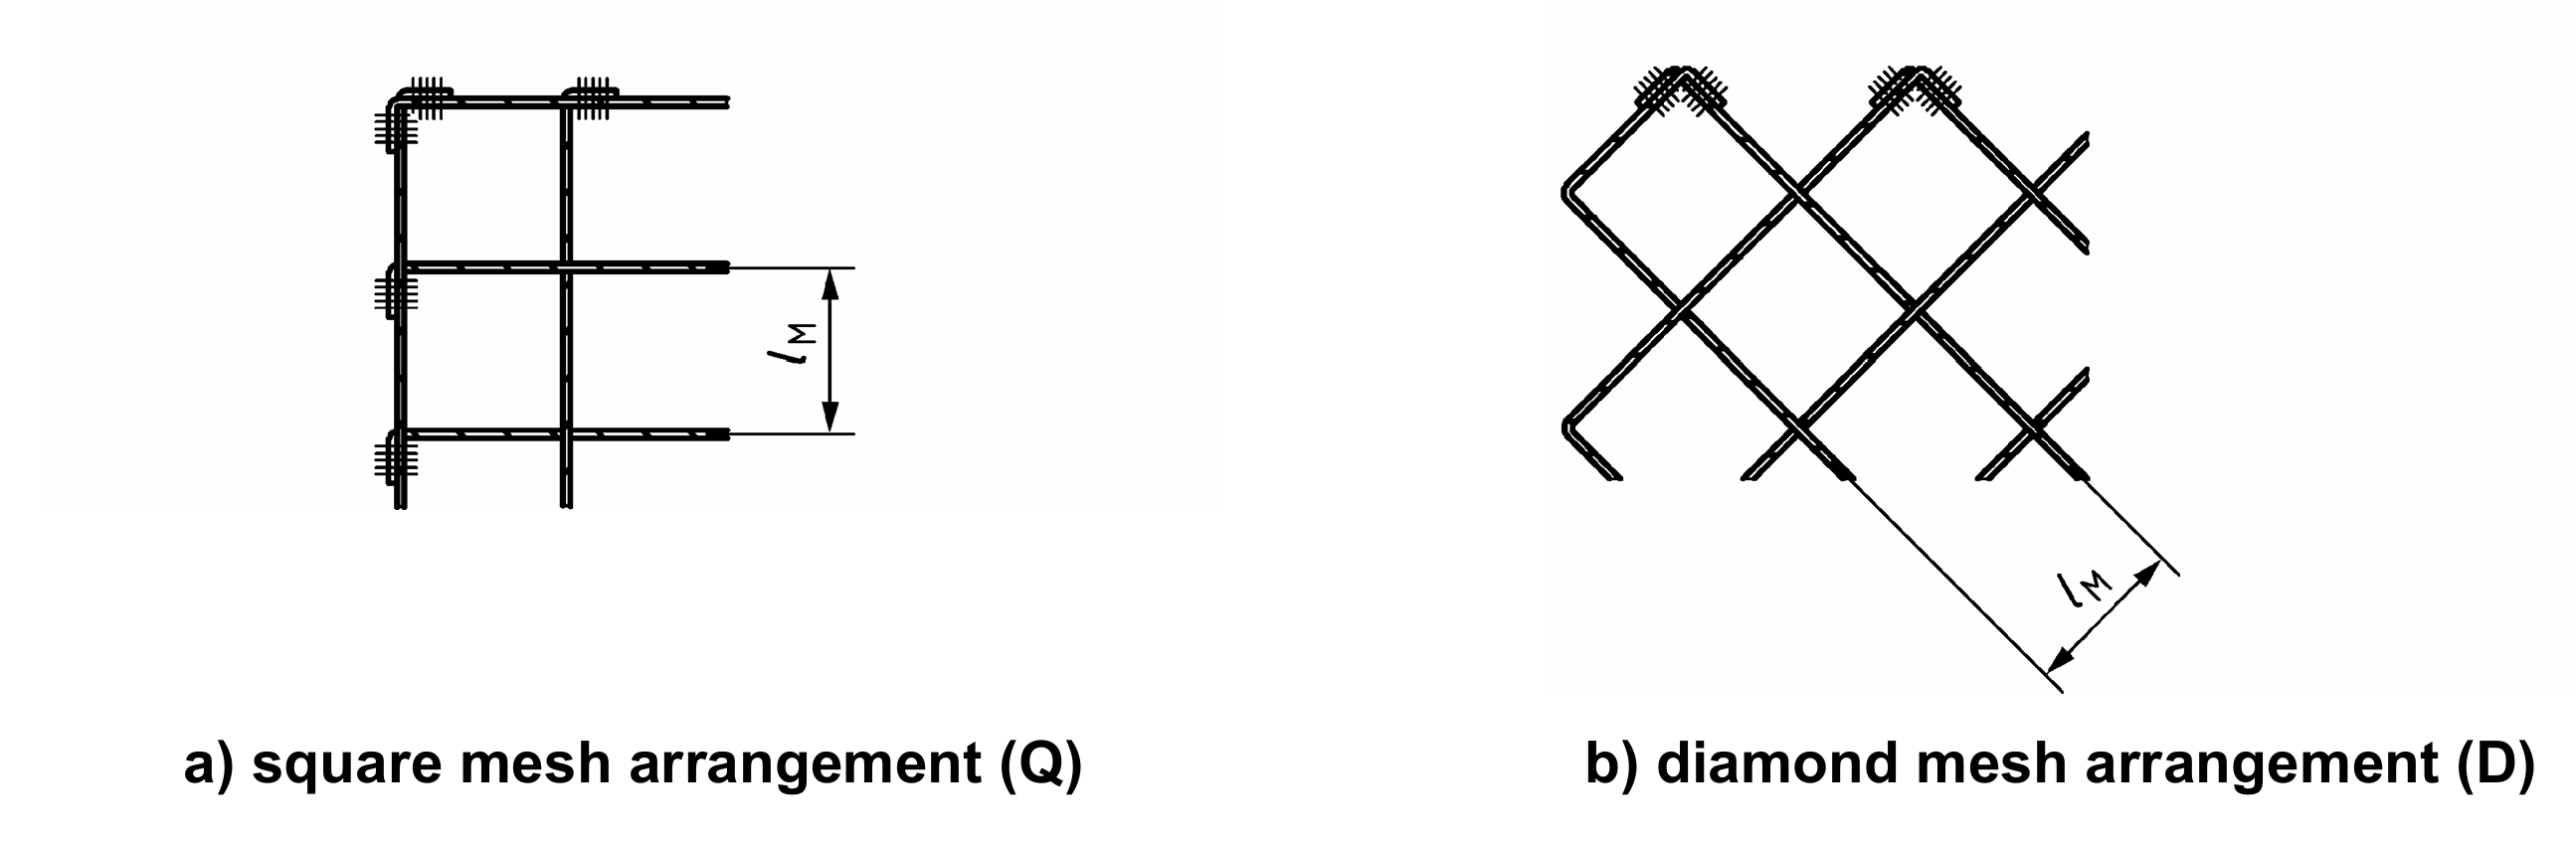
\includegraphics[height=0.2\textheight, keepaspectratio]{143_capitoli/capitolo1/immagini_capitolo_1/geometria_reti.png}
    \caption{Geometrie delle maglie di rete possibili secondo la norma EN 1263-1. Fonte: BS EN 1263-1}
    \label{fig:geometria_reti}
\end{figure}

Dal punto di vista del processo produttivo e del comportamento dissipativo locale, le reti si dividono in due categorie principali:
\begin{itemize}
    \item \textit{Reti con nodo (knotted nets):} Le maglie sono realizzate annodando meccanicamente i filamenti nei punti. Durante la fase iniziale di un impatto dinamico, il serraggio progressivo dei nodi sotto trazione costituisce un importante meccanismo di dissipazione di energia, prima dell'innesco della risposta elastoplastica del filamento sintetico. 
    \item \textit{Reti senza nodo (knotless nets):} Realizzate mediante processi di tessitura continua, in cui i trefoli si compenetrano nei punti di incrocio senza la presenza di nodi fisici. Questa tecnologia elimina i picchi di usura per sfregamento locale e riduce la concentrazione di sforzi nei punti di intersezione, modificando parzialmente la risposta dissipativa del sistema che si affida quasi esclusivamente alla deformazione del materiale polimerico impiegato. 
\end{itemize} 

\subsubsection{Degrado del materiale ed effetti dell'invecchiamento}
I filamenti sintetici in poliammide (PA), in polipropilene (PP) o in polietilene (PE) che costituiscono i trefoli delle reti di sicurezza sono soggetti a un progressivo degrado delle proprietà meccaniche a causa dell'esposizione prolungata agli agenti atmosferici. Dalla letteratura sul tema emerge come tra i fattori ambientali più penalizzanti vi siano: 
\begin{itemize}
    \item \textit{Radiazione solare:} La radiazione solare rappresenta la principale causa di invecchiamento per le fibre sintetiche delle funi. Sebbene la frazione ultravioletta (UV) costituisca solo una piccola parte dello spettro solare complessivo che raggiunge il suolo, è proprio la sua elevata energia a guidare il processo di degrado, provocando un infragilimento della fibra con conseguente riduzione della resistenza a trazione, della deformabilità a rottura e della capacità di assorbimento dell'energia elastica. In merito a tale effetto, la normativa prescrive che lo spettro di emissione della sorgente luminosa impiegata nei test di invecchiamento artificiale (\textit{artificial ageing test}) sia compreso all'interno del campo dell'ultravioletto (UV).
    \item \textit{Variazioni termiche:} La escursioni termiche ambientali (sia giornaliere che stagionali) provocano continui cicli di dilatazione e concentrazione microscopica nei filamenti. Inoltre, l'aumento della temperatura esercita un effetto sinergico con la radiazione solare, accelerando il processo di degradamento delle proprietà meccaniche. 
    \item \textit{Cicli igrometrici:} Le variazioni dell'umidità relativa dell'aria determinano continui processi di assorbimento e rilascio di vapore acqueo nella matrice polimerica. Tali cicli igrometrici generano stati tensionali alternati all'interno della fibra che favoriscono la formazione di micro-fessurazioni superficiali. 
    \item \textit{Azione dell'acqua:} L'esposizione diretta alle intemperie e i ripetuti cicli di bagnamento e asciugatura provocano il progressivo dilavamento degli additivi chimici stabilizzanti e dei protettivi UV inseriti nella fibra durante la produzione, provocando l'accelerazione dei fenomeni di degrado. 
\end{itemize}

Per garantire che la rete mantenga i requisiti minimi di sicurezza durante l'operatività in cantiere, la norma \cite{EN1263-1} definisce la durabilità standard del dispositivo e impone la presenza nella rete in opera di campioni di rete (\textit{test mesh}) appartenenti allo stesso lotto di produzione. Tali campioni estraibili consentono di verificare sperimentalmente, su base annuale, la resistenza residua a trazione secondo la prova definita dalla norma EN ISO 1806 \cite{ENISO1806-2002}, al fine di autorizzarne l'eventuale prolungamento d'impiego.

Ai fini della modellazione ad elementi finiti trattata successivamente, l'effetto del degrado per invecchiamento ambientale non verrà preso in considerazione. Le analisi numeriche assumeranno il materiale della rete nello stato nominale di fornitura, consentendo di isolare il comportamento meccanico puro.

\subsection{Reti anticalcinacci}
\begin{figure}[htbp]
    \centering
    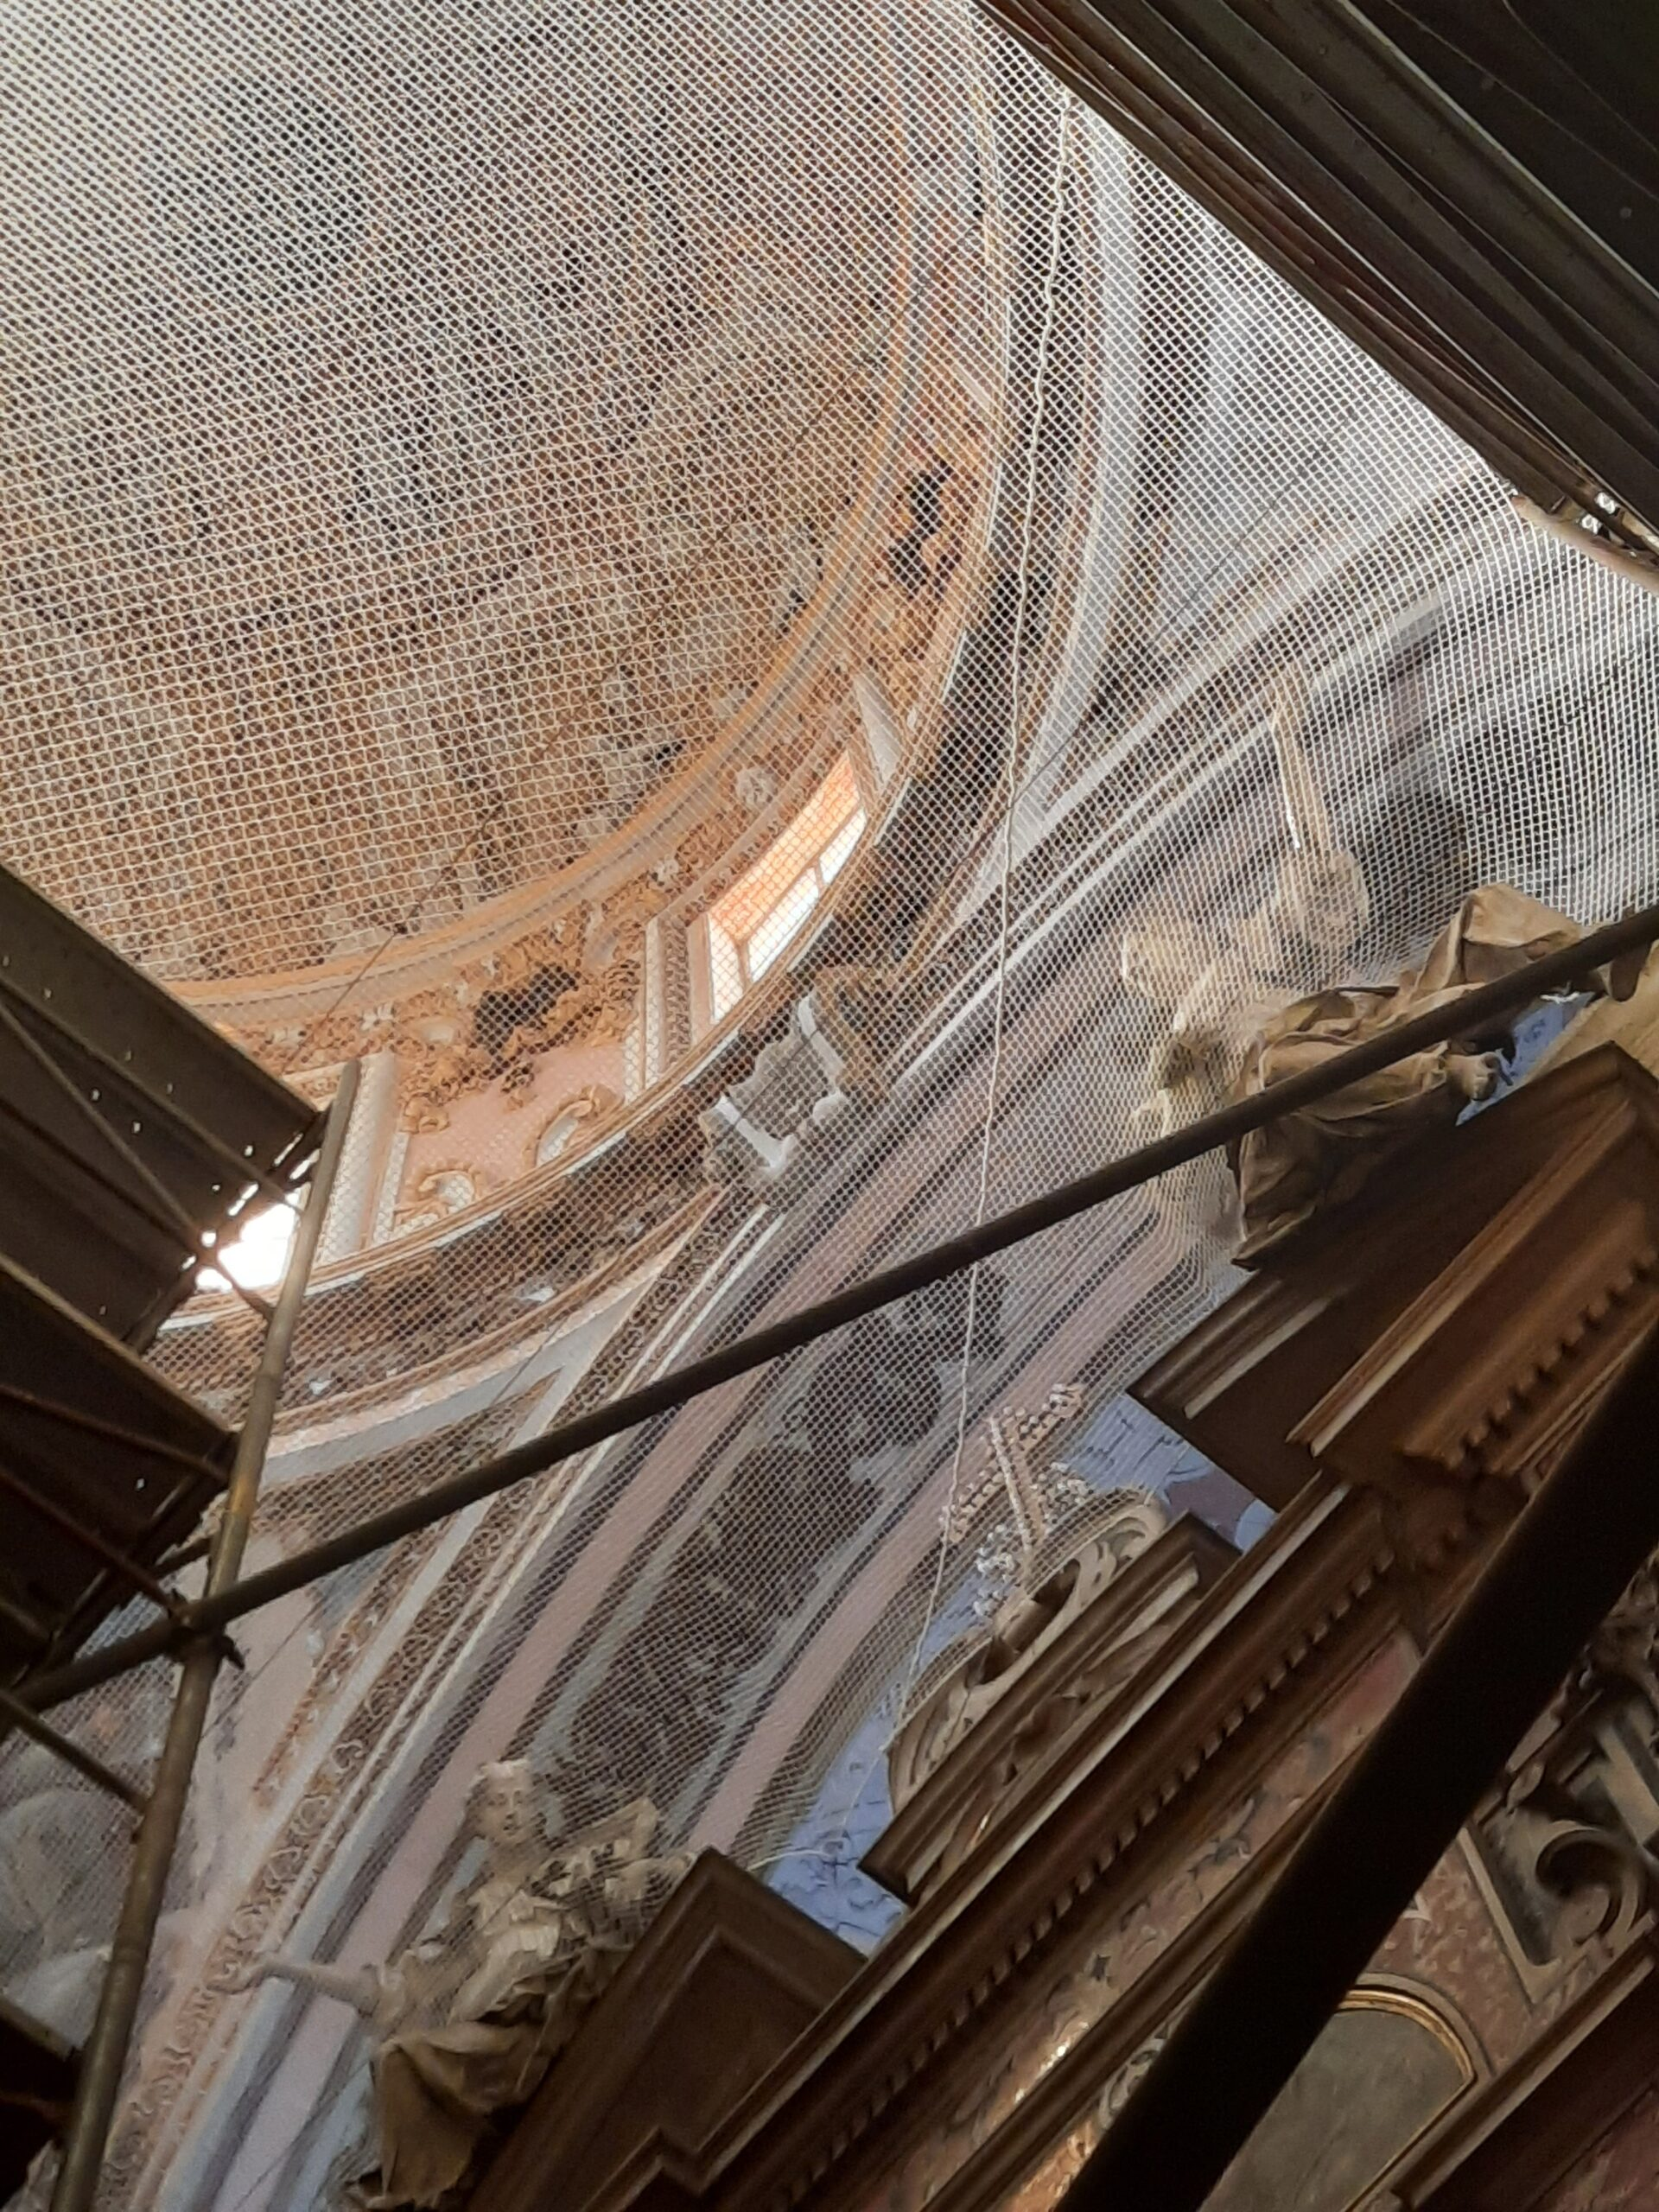
\includegraphics[height=0.35\textheight, keepaspectratio]{143_capitoli/capitolo1/immagini_capitolo_1/rete_anticalcinacci_3.jpg}
    \caption{Installazione di una rete anticalcinacci a protezione degli ambientiinterni in un edificio di culto. Fonte: www.laretesrl.it}
    \label{fig:rete_anticalcinacci1}
\end{figure}
\begin{figure}[htbp]
    \centering
    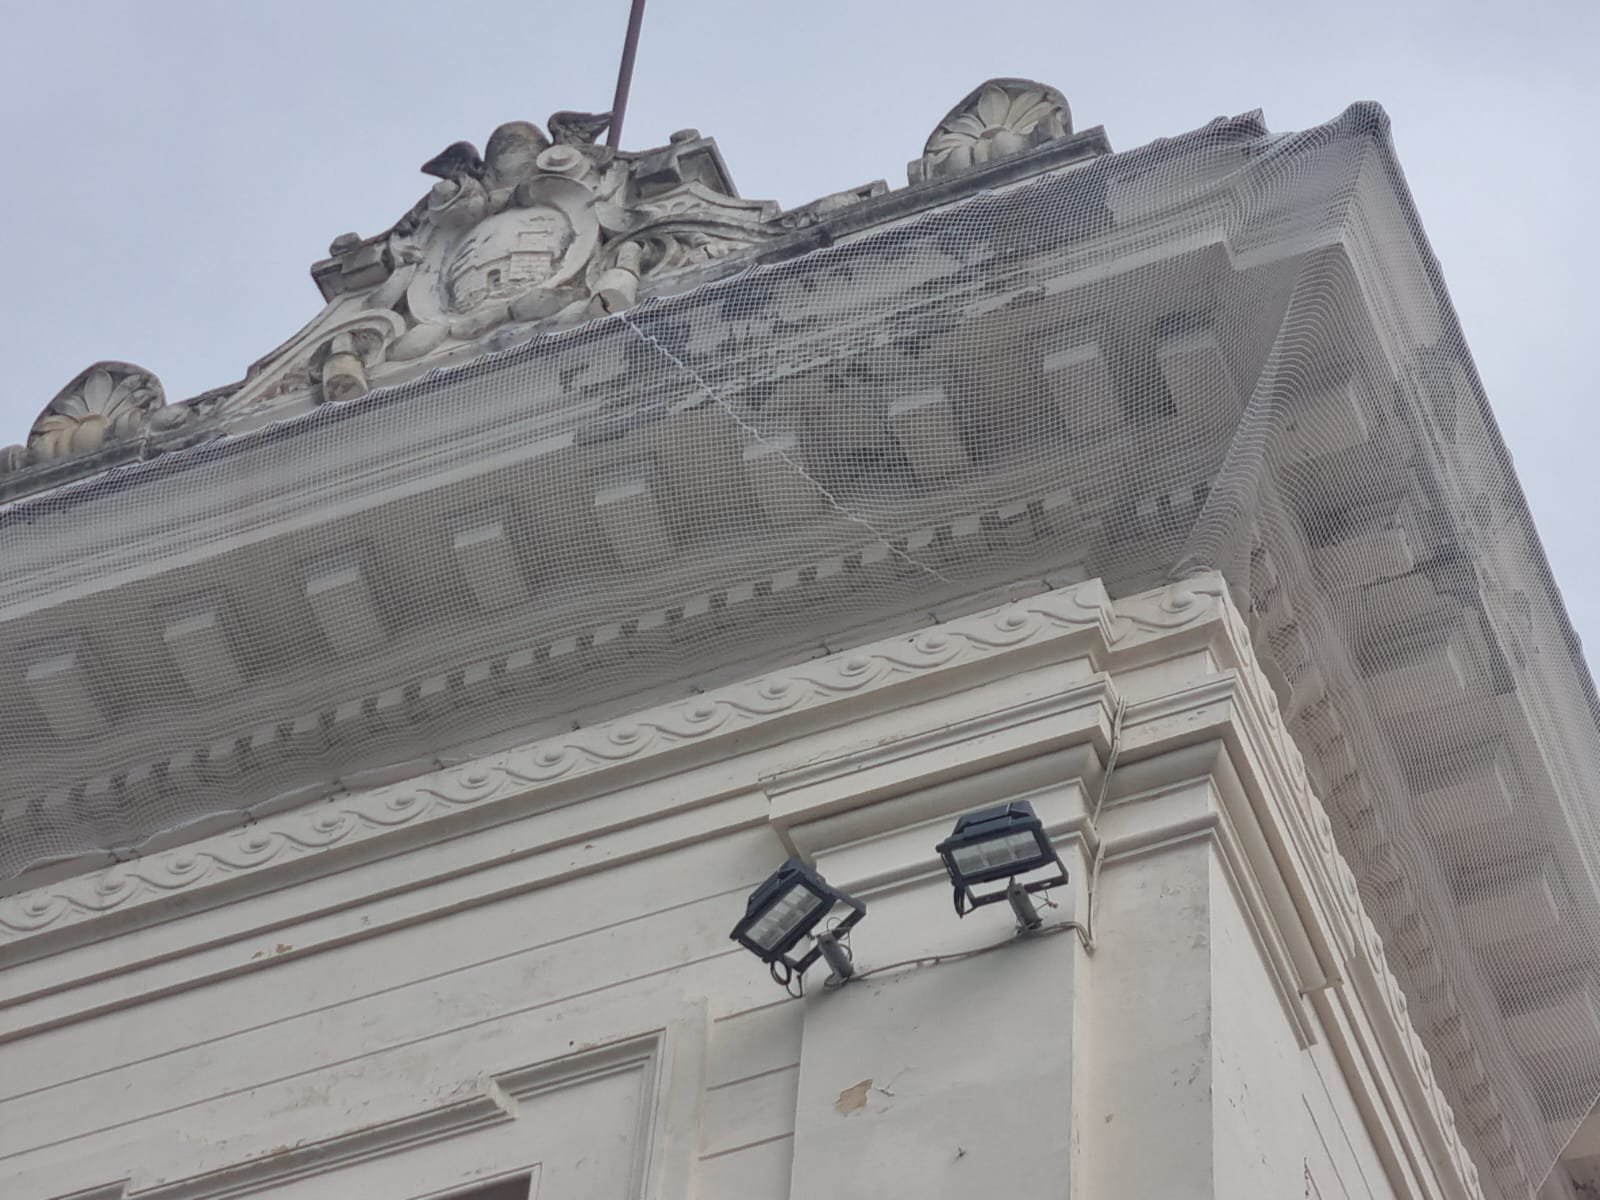
\includegraphics[height=0.35\textheight, keepaspectratio]{143_capitoli/capitolo1/immagini_capitolo_1/rete_anticalcinacci_4.jpg}
    \caption{Messa in opera di una rete anticalcinacci per la protezione perimetrale aderente alla modanatura di facciata. Fonte: www.laretesrl.it}
    \label{fig:rete_anticalcinacci2}
\end{figure}
Le reti anticalcinacci ed antidetriti rappresentano dei dispositivi di sicurezza fondamentali, soprattutto in contesti urbani e industriali, dove la presenza di edifici in fase di ristrutturazione, facciate degradate e strutture sopraelevate può comportare pericoli per persone e cose. 

A differenza delle reti di sicurezza per la protezione nei confronti dal rischio di caduta delle persone, i dispositivi destinati al solo contenimento di materiali ed oggetti sono regolamentati in Italia dalle parti specifiche della serie UNI 11808, ossia la \cite{UNI11808-3} per i requisiti prestazionali e di prova e la \cite{UNI11808-4} per le prescrizioni di posa e uso. 

La principale differenza geometrica e funzionale tra una rete anticalcinacci e un sistema di protezione primario per le persone risiede nella dimensione nominale della maglia $l_m$ che, in questo caso, risulta essere notevolmente più fitta ($l_m = 10 \div 25 \, \text{mm}$) o una struttura microforata. Tale riduzione della luce netta è indispensabile per impedire fisicamente il passaggio di elementi di piccola pezzatura, a fronte di una capacità di assorbimento energetico globale decisamente inferiore. La norma distingue così due configurazioni principali: 
\begin{itemize}
    \item \textit{Sistema O1A:} rete combinata con telo;
    \item \textit{Sistema 01B:} rete senza telo.
\end{itemize}

In cantiere, l'impiego di reti di questo tipo avviene principalmente secondo due configurazioni:
\begin{itemize}
    \item \textit{Integrazione su reti anticaduta primarie:} La rete antidetriti a maglia fitta conforme alla \cite{UNI11808-3} viene sovrapposta e legata direttamente ad una rete di sicurezza principale. In questo schema la rete primaria regolata dalla \cite{EN1263-1} assorbe la quota prevalente dell'energia di impatto di corpi voluminosi, mentre la rete secondaria trattiene i detriti con diametro nominale inferiore.
    \item \textit{Rivestimento continuo di facciate e ponteggi:} La rete viene tesa a copertura perimetrale dell'opera o dei telai del ponteggio per contenere la dispersione di polveri ed il distacco di calcinacci.
\end{itemize}

In fase di progettazione delle strutture di sostegno e delle opere provvisionali, la posa di reti anticalcinacci impone di tener conto l'azione del vento. A causa della ridotta porosità della maglia fitta, la rete genera una resistenza aerodinamica non trascurabile che si traduce in rilevanti spinte orizzontali. Ai sensi della norma sui ponteggi \cite{UNI12811-1}, tali azioni aerodinamiche devono essere opportunamente calcolate in funzione dell'effettiva superficie ostruita dal telo o dalla rete, al fine di verificare la stabilità globale della strutture e la tenuta degli ancoraggi.

\subsection{Barriere e reti paramassi}
I fenomeni di crollo roccioso rappresentano una delle tipologie di dissesto idrogeologico più insidiose e ad alto rischio per le infrastrutture viarie, i centri abitati ed i cantieri in territorio montano. La spiccata cinematica del fenomeno, caratterizzata da elevate velocità di propagazione e traiettorie complesse, richiede la progettazione di sistemi di protezione. 

Nell'ambito dell'ingegneria geotecnica ed in maniera più specifica riguardo alla stabilità dei pendii rocciosi, le opere di mitigazione del rischio da caduta massi si dividono in due macro-categorie: 
\begin{itemize}
    \item \textit{Sistemi di protezione attiva:} sono opere applicate direttamente sulla parete rocciosa per prevenirne il distacco o stabilizzare i blocchi potenzialmente instabili (es. reti in fune d'acciaio, tiranti e chiodature, cortine ad aderenza migliorata). 
    \item \textit{Sistemi di protezione passiva:} sono opere interposte lungo la traiettoria di caduta del blocco con la funzione di intercettare, arrestare o deviare la messa in movimento dopo il distacco (es. barriere paramassi a rete, rilevati paramassi, gallerie artificiali di protezione contro la caduta dei massi). 
\end{itemize}

\begin{figure}[htbp]
    \centering
    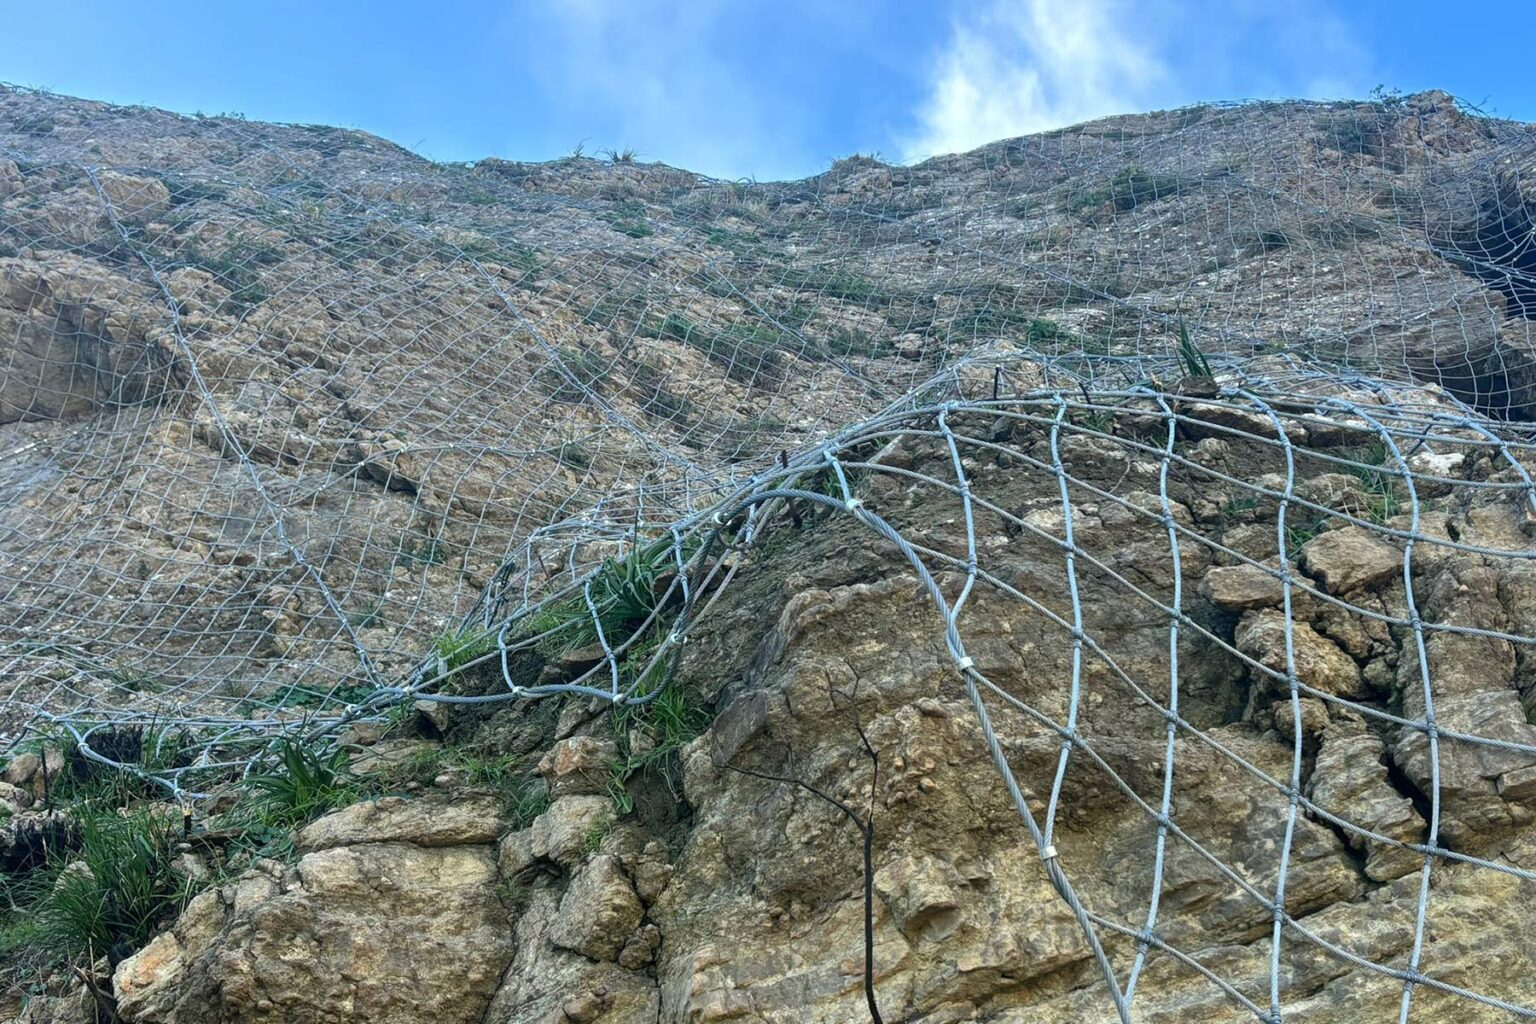
\includegraphics[height=0.35\textheight, keepaspectratio]{143_capitoli/capitolo1/immagini_capitolo_1/misure_attive_versanti_rocciosi.jpg}
    \caption{Sistemi di protezione attiva, rafforzamento corticale su versante roccioso. Fonte: www.maccaferrisicilia.com}
    \label{fig:misure_attive_versanti_rocciosi}
\end{figure}

\begin{figure}[htbp]
    \centering
    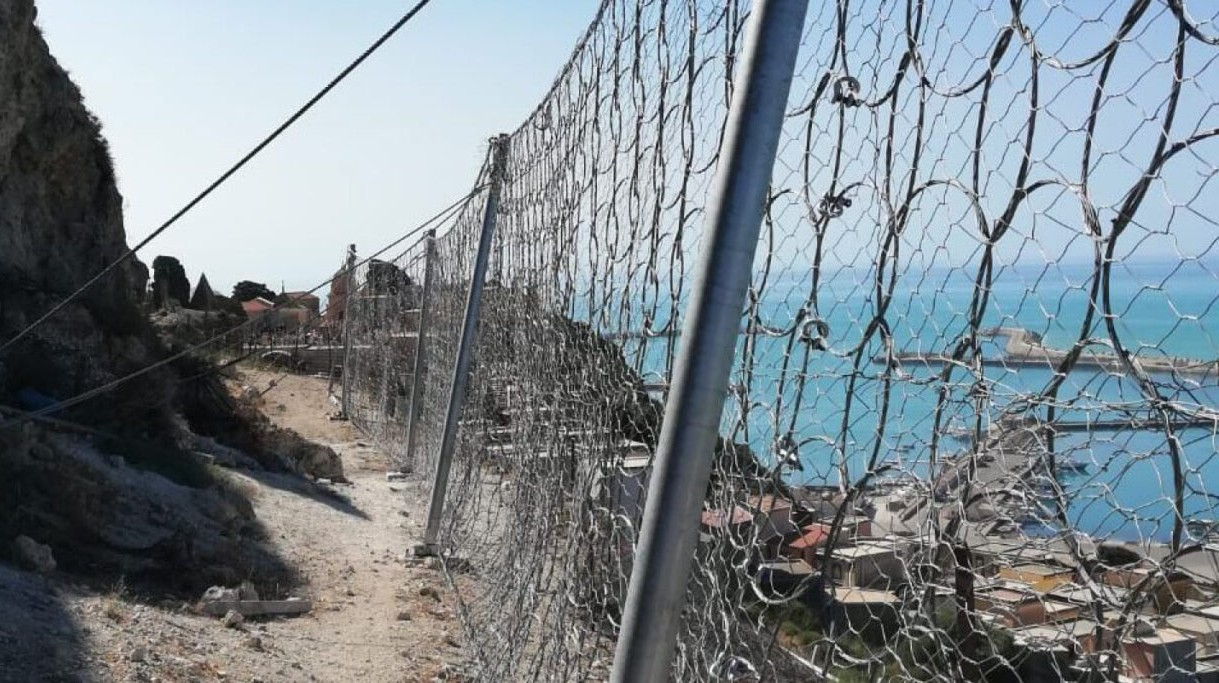
\includegraphics[height=0.35\textheight, keepaspectratio]{143_capitoli/capitolo1/immagini_capitolo_1/barriere_paramassi_1_b.jpg}
    \caption{Sistemi di proteziozione passiva, installazione di una barriera paramassi. Fonte: www.maccaferrisicilia.com}
    \label{fig:barriere_paramassi_figura}
\end{figure}

\'E proprio nell'ambito dei sistemi di protezione passiva - e in particolare delle barriere paramassi - che si possono trovare applicazioni del presente lavoro di tesi. Il meccanismo resistente fondamentale di tali strutture è infatti governato dall'interazione dinamica e dalla capacità di sviluppare elevate deformazioni fuori dal piano della rete a seguito dell'urto.

La prestazione dei sistemi di barriere paramassi è espressa in termini del massimo livello di energia assorbibile (\textit{Maximum Energy Level - MEL}). Poichè l'energia di dissipazione è correlata all'accumulo di deformazioni permanenti del sistema, la classificazione delle barriere può essere definita anche in funzione della sua deformabilità: maggiore è lo sviluppo di deformazioni plastiche, superiore sarà la capacità di assorbimento della barriera. Nel caso in cui i sistemi siano in grado di dissipare elvati valori di energia di impatto (fino a $8000 \, \text{kJ}$ e oltre), si parla di barriere flessibili ad alto assorbimento di energia. Al contrario, in presenza di sistemi meno deformabili con una ridotta capacità di dissipazione, ci si riferisce a barriere rigide e semirigide.

Il comportamento di una sistema di barriere paramassi è traduzionalmente classificato in funzione dei risultati di prove a piena scala, nelle quali un prototipo è soggetto all'impatto di un blocco aventi massa e velocità prestabilite. In Europa la linea guida è stata sviluppata \cite{EAD-FRK} per fornire una procedura standardizzata per valutare le performance attraverso tali esperimenti, con lo scopo di avere uno standard uniforme per la qualificazione dei prodotti commerciali.

\begin{figure}[htbp]
    \centering
    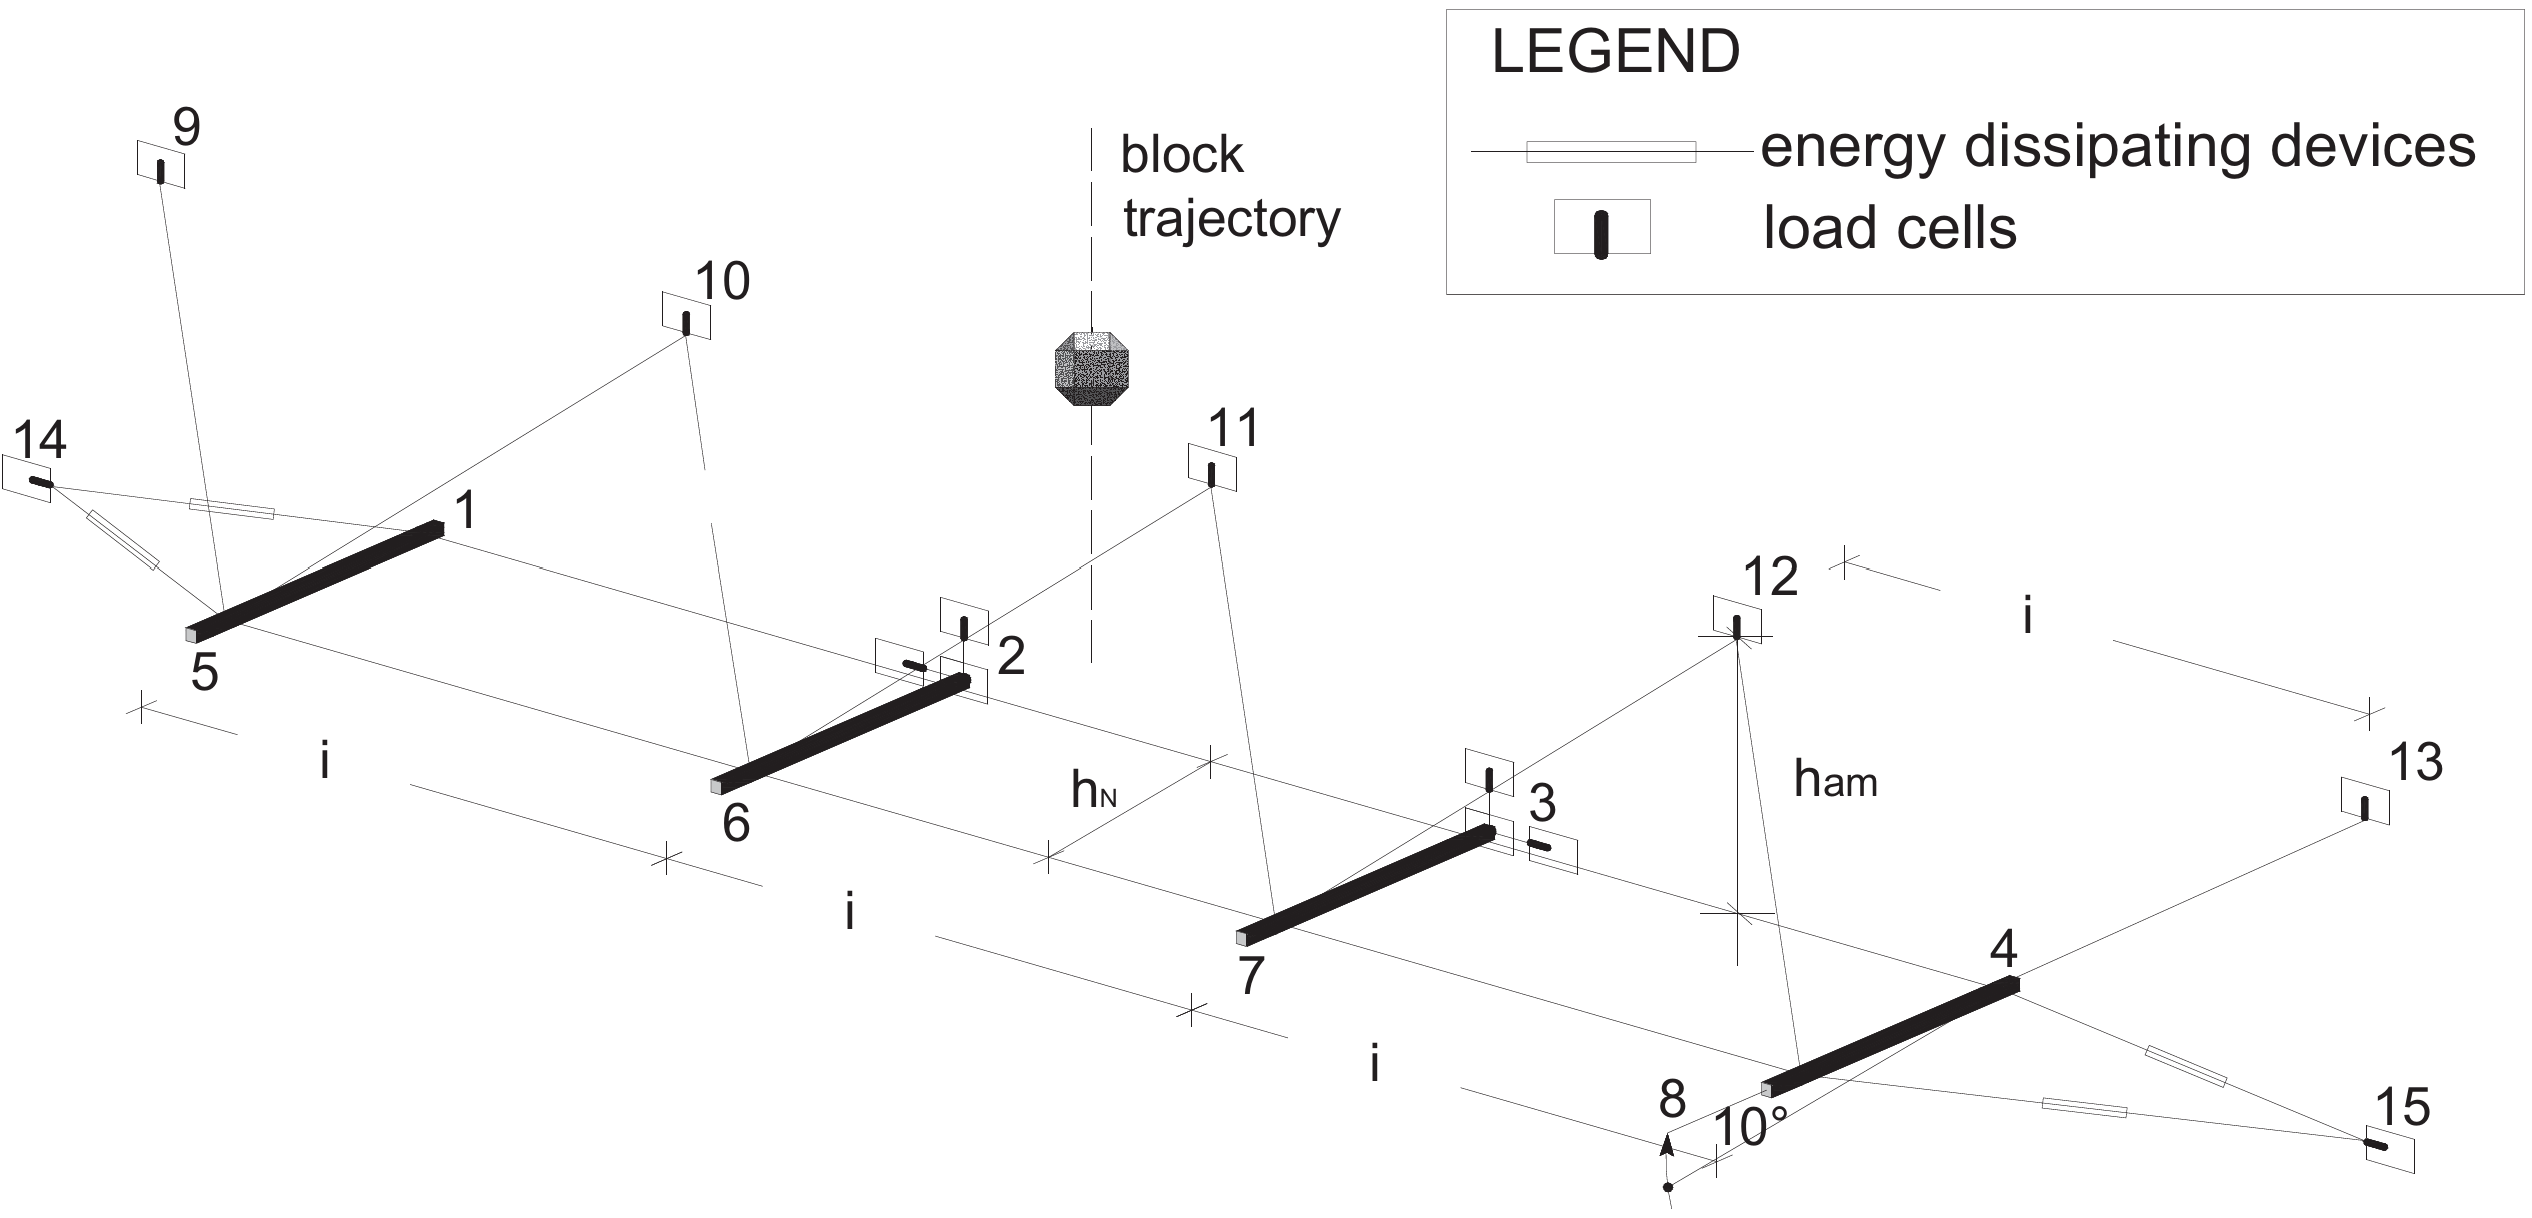
\includegraphics[height=0.30\textheight, keepaspectratio]{143_capitoli/capitolo1/immagini_capitolo_1/schema_di_prova_gentilini.png}
    \caption{Schematizzazione del layout geometrico a tre campate di una barriera paramassi, con indicazione della traiettoria del blocco, dei dissipatori e della posizione delle celle di carico (tratto da \cite{gentilini2012}).}
    \label{fig:barriere_paramassi_schema_prova}
\end{figure}

La normativa impone l'esecuzione di test dinamici in vera grandezza su un kit completo di barriera, comprensivo di:
\begin{itemize}
    \item \textit{Struttura di intercettazione:} è la rete metallica che può avere varie geometrie (romboidale \cite{EAD230006}, esagonale, ad anello \cite{EAD230005}). La sua funzione è quella di intercettare e fermare il blocco di roccia in caduta. La rete ha il compito di reggere all'impatto diretto di un corpo, assorbendo la maggior parte della sua energia cinetica derivante dall'evento attraverso deformazioni elastoplastiche.
    \item \textit{Struttura di supporto:} è costituita da elementi in acciaio di varie tipologie di sezione. Sono progettati per mantenere in posizione la struttura di intercettazione e per trasmettere le forze risultanti dall'impatto alle fondazioni.
    \item \textit{Componenti di connessione:} sono generalmente cavi, dispositivi di dissipazione dell'energia, perni, morsetti e tutti gli altri elementi impiegati all'intersezione dei nodi per le connessioni interni tra le varie parti costitutive. Hanno la funzione di connettere la rete alle strutture di supporto e di trasmettere le sollecitazioni derivanti dall'impatto, alle fondazioni. 
    \item \textit{Sistema di fondazione:} generalmente sono progettate come piastre di base per i pali o per i sistemi di ancoraggio a terra dei cavi. Devono essere progettate per distribuire i carichi derivanti dagli impatti al terreno senza raggiungere la rottura, che provocherebbe il ribaltamento della barriera.
\end{itemize}

La prova dinamica si basa su un principio analogo a quello previsto dalle normative per le reti di sicurezza: un peso viene lanciato in scala reale sul sistema per valutarne la capacità di arresto e dissipazione.

Attorno all'esecuzione di queste prove sperimentali in vera grandezza si è sviluppata negli anni un'ampia e consolidata letteratura scintifica basata sulla simulazione mediante modelli agli elementi finiti (FEM). Poichè i test fisici al massimo livello di energia (MEL) comportano costi estremamente elevati, infrastrutture complesse e la distruzione dei prototipi, la modellazione numerica si è affermata come uno strumento fondamentale per analizzare nel dettagli la risposta dinamica non lineare dell'intero kit di protezione \cite{gentilini2012,gentilini2013},

Oltre alle prove dinamiche a piena scala previste per la qualificazione dell'intero kit di barriera, la caratterizzazione meccanica del singolo pannello di rete trova un importante riferimento nella norma \textit{UNI 11437:2012} \cite{UNI11437-3}. Tale standard definisce la procedura di prova per sollecitare quasi-staticamente un singolo pannello di rete mediante un punzone semisferico applicato ortogonalmente al piano della maglia, fornendo un riferimento chiaro per la determinazione della sua capacità di assorbimento dell'energia.

È proprio in questo contesto che si inserisce il presente lavoro di tesi, la cui attenzione viene focalizzata sullo sviluppo di un software di calcolo FEM in grado di quantificare l'energia assorbibile dalla rete sotto forma di energia potenziale elastica. Questa misura potrebbe inizialmente sembrare fuori contesto rispetto alle richieste convenzionali delle normative a piena scala; tuttavia, come verrà mostrato nel \cref{chap:capitolo3}, tale parametro rappresenta una condizione sufficiente a decretare il fallimento del sistema di intercettazione dei corpi, consentendo di scartare a priori i casi che non soddisfano i requisiti minimi.

Nel presente studio, l'applicazione del codice viene condotta su elementi in polietilene sollecitati secondo la logica della prova di punzonamento; tuttavia, vista la generalità del modello, la metodologia potrà essere estesa anche ad elementi metallici con caratteristiche geometriche analoghe o modellabili con le stesse assunzioni introdotte nel software (un esempio di modellazione di \textit{wire ring mesh} con elementi asta equivalenti è proposto in \cite{gentilini2013}).

\subsection{Applicazioni architettoniche}

\section{Altre applicazioni}



